\begin{figure}[!tb]
\begin{center}
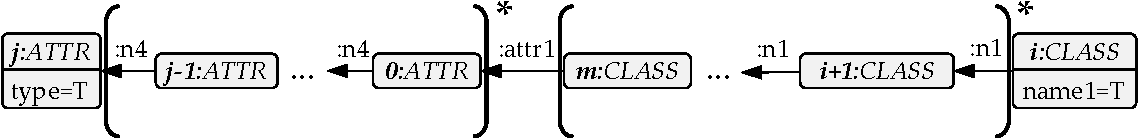
\includegraphics[width=.9\textwidth]{img/software_trans/rec_graph.pdf}
\end{center}
\caption{Language of Recursive Graph Schemata}
\label{fig:sec-compl-software-trans:rec_graph_lang}
\end{figure}

We introduce recursive conditions as a special class of infinite conditions and show that it is sufficient to check the components of the recursions only to verify domain completeness of the whole system.
Recursive conditions are infinite conditions that are given by the disjunction over the infinite set of graphs that are obtained from a start (premise) graph by repeating specific graph structures recursively.
In particular, this allows the definition of conditions over regular paths in abstract syntax graphs of source code.
\cref{fig:sec-compl-software-trans:rec_graph_lang} illustrates such a regular path expression defining that there is some path between an \code{ATTR}ibute $j$ of \code{type} $T$ and the \code{CLASS} $i$ with name $T$.
Concretely,
\begin{enumerate*}
\item[a)] either $j$ is directly connected to $i$ via edge \code{:attr1}, i.e., $j$ is the first attribute of class $i$, or
\item[b)] $j$ is the $j$th attribute of class $i$ and there are $j-1$ other attributes between both via \code{:n4} edges, or
\item[c)] $j$ is the first attribute of some other class $m$ and there are $m-i$ other classes between $i$ and $m$ via \code{:n1} edges, or
\item[d)] $j$ is the $j$th attribute of class $m$ and $m$ is the $m-i$th class defined behind class $i$.
\end{enumerate*}
Therefore, we want to describe an infinite set of graphs (paths) where the graph (path) structures that are enclosed by brackets with the Kleene star $*$ may be repeated recursively.
This allows the definition of the constraint ``Each attribute $j$ of type $T$ is the attribute of some class $m$ and moreover, for each such $j$ there is a class $i$ with name $T$ and either $i=m$ or $i$ is defined somewhere before $m$.'' - condensed ``For each attribute type that is used there is a corresponding class definition.''.
Such a constraint is rather an infinite constraint, i.e., the disjunction over all possible paths between $j$ and $i$. 
Thus, the motivation behind the notion of recursive conditions (constraints) is
\begin{enumerate*}
\item[a)] to have a notation for defining infinite graph conditions with recursively repeating graph structures,
\item[b)] and whose satisfiability is decidable,
\item[c)] the ability to involve infinite graph constraints in verifying domain completeness while in general, the verification of domain completeness for infinite constraints does not terminate, and
\item[d)] in particular, to use recursive graph constraints for specifying constraints over regular paths for the definition of abstract syntax graphs.
\end{enumerate*}
We introduce the notion of recursive graph schemata for the definition of infinite sets of graphs that are obtained from a start graph by the (recursively repeated) restricted application of productions via pre-defined matches between the productions.
 
\begin{definition}[Recursive Graph Schema]
\label{def:sec-compl-software-trans:rec_cond}
A \emph{recursive graph schema}\index{recursive graph schema} $\GS=(\GG,M,s_\GS,t_\GS)$ is given by
\begin{enumerate}
  \item a graph grammar $\GG=(S,P)$ with start graph $S$ and a set $P$ of productions $p=(L_p \transB{l_p} K_p \trans{r_p} R_p)$ with LHS $L_p$, gluing object $K_p$, RHS $R_p$ and $l_p,r_p \in \M$,
  \item a set $M$ of matches $m \in \M$ where
  \begin{enumerate}
    \item $m\colon L_p \to S$ from the LHS $L_p$ of some $p \in P$ to start graph $S$, or
    \item $m\colon L_p \to R_{p'}$ from the LHS $L_p$ of some $p \in P$ to the RHS $R_{p'}$ of some $p' \in P$, and
  \end{enumerate}
  \item source function $s_\GS\colon M \to P$ and target function $t_\GS\colon M \to (S \cup P)$ such that for all $m \in M$, $s_\GS(m\colon L_p \to A)=p$ and furthermore, $t_\GS(m\colon A \to S)=S$ or $t_\GS(m\colon A \to R_p)=p$ for some $p=(L_p \gets K_p \to R_p) \in P$.\envEndMarker
\end{enumerate} 
\end{definition}

\begin{remark}[Recursive Graph Schema]
Note that by function $s_\GS$, each match is mapped to exactly one rule as source (analogously, with $t_\GS$ for the target).
However, this does not restrict the expressiveness of recursive graph schemata.
Two rules $p_1\colon L \gets K_1 \to R_1,p_2\colon L \gets K_2 \to R_2$ with the same LHS $L$ and the same outgoing match $m\colon L \to A$ can be redefined by two rules $p_1,p'_2\colon L' \gets K_2 \to R_2$ with distinct LHSs $L \neq L'$ and distinct matches $m,m'\colon L' \to A$ by renaming the elements (nodes and edges) of $L$ resulting in $L'$ and without changing the semantics up to isomorphism.
This allows to define separate sources for $m,m'$ with $s_\GS(m)=p_1$ and $s_\GS(m')=p'_2$.
\envEndMarker
\end{remark}

\begin{figure}[!tb]
\begin{center}
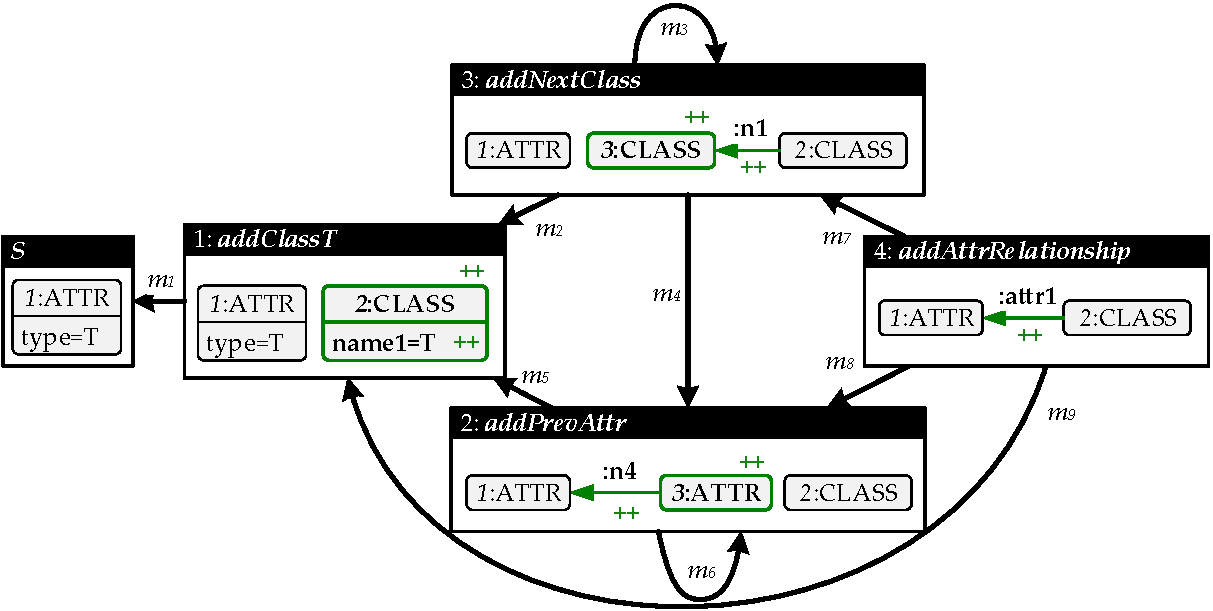
\includegraphics[width=.95\textwidth]{img/software_trans/graph_schema.pdf}
\begin{math}
m_1=(1 \mapsto 1); m_2=(1 \mapsto 1,2 \mapsto 2); m_3=(1 \mapsto 1,2 \mapsto 3); m_4=(1 \mapsto 3,2 \mapsto 2);m_5=(1 \mapsto 1,2 \mapsto 2);m_6=(1 \mapsto 3,2 \mapsto 2);m_7=(1 \mapsto 1,2 \mapsto 3);m_8=(1 \mapsto 3,2 \mapsto 2);m_9=(1 \mapsto 1,2 \mapsto 2)
\end{math}
\begin{math}
s_\GS(m_1)=\code{1:addClassT};s_\GS(m_2)=s_\GS(m_3)=s_\GS(m_4)=\code{3:addNextClass};s_\GS(m_5)=s_\GS(m_6)=\code{2:addPrevAttr};s_\GS(m_7)=s_\GS(m_8)=s_\GS(m_9)=\code{4:addAttrRelationship};
\end{math}
\begin{math}
t_\GS(m_1)=S;t_\GS(m_2)=t_\GS(m_5)=t_\GS(m_9)=\code{1:addClassT};t_\GS(m_3)=t_\GS(m_7)=\code{3:addNextClass};t_\GS(m_4)=t_\GS(m_6)=t_\GS(m_8)=\code{2:addPrevAttr};
\end{math}
\end{center}
\caption{Recursive Graph Schema}
\label{fig:sec-compl-software-trans:rec_graph}
\end{figure}

\begin{example}[Recursive Graph Schema]
\label{ex:sec-compl-software-trans:rec_schema}
\cref{fig:sec-compl-software-trans:rec_graph} illustrates a recursive graph schema with start graph $S$, productions $\{1 \ldots 4\}$, matches $\{m_1 \ldots m_9\}$ and source (target) function $s_\GS$ ($t_\GS$) which defines the infinite set of graphs that are presented in \cref{fig:sec-compl-software-trans:rec_graph_lang}.
From start graph $S$ we obtain the graph with the corresponding \code{CLASS} of name $T$ and edge \code{:attr1} by applying rules \code{1} and \code{4} via matches $m_1$ and $m_9$ successively.
Analogously, we may obtain bigger graphs beginning with $S$ by (repeatedly) applying rules \code{2} and \code{3} via corresponding matches $m_2 \ldots m_6$ before applying rule \code{4}.
Note that cycles of match morphisms define graph structures that may be repeated recursively.
The repeated application of rule~\code{3} via match $m_3$ allows the repeated addition of classes whereas rule~\code{2} together with match $m_6$ allows the repeated addition of attributes.
\envEndMarker
\end{example}

We define the precise semantics of a recursive graph schema $\GS$ by its graph language which is induced by terminating recursive transformation sequences over the schema starting at start graph $S$.
A recursive transformation sequence is given by a path of matches $M$ in $\GS$ and a corresponding sequence of recursive transformation steps where the match of each step is restricted by the co-match of the previous step.
The sequence is terminating in the sense that there are no matches defined in $M$ for extending the sequence.
A path of matches $M$ in $\GS$ is given by a sequence of matches $(m_i \in M)_{i \in I}$ with $s_\GS(m_i)=t_\GS(m_{i+1})$, for all $i \in I$.

\begin{definition}[Cyclic \& Terminating Match-Path]
\label{def:sec-compl-software-trans:c_t_match-path}
Let $\GS=((S,P),M,s_\GS,t_\GS)$ be a recursive graph schema.
A \emph{match-path in $\GS$}\index{match-path} is a sequence of $n>0$ matches $(m_i \in M)_{i \in I},I=\{1 \ldots n\}$ with $s_\GS(m_i)=t_\GS(m_{i+1})$, for all $i \in I$.
A match-path with $n$ matches is \emph{terminating}\index{match-path!terminating}, if there does not exist a match $m \in M$ with $t_\GS(m)=s_\GS(m_n)$.
A match-path is \emph{acyclic}\index{match-path!acyclic}, if for all $i,j \in I$ it is true that $i \neq j$ implies $s_\GS(m_i) \neq s_\GS(m_j)$.
Otherwise, the match-path is \emph{cyclic}\index{match-path!cyclic}.
A match-path of $n$ matches \emph{starts (ends)}\index{match-path!starts in}\index{match-path!ends in} in $A$, if $t_\GS(m_1)=A$ ($s_\GS(m_n)=A$).
With $\Paths_A(\GS)$ we denote \emph{the set of all match-paths in $\GS$ that start in $A$} and with $\Paths_{A,B}(\GS)$ we denote \emph{the set of all match-paths in $\GS$ that start in $A$ and end $B$}\index{match-path!set of paths}.
A \emph{match-cycle is some match-path $\paths \in \Paths_{A,A}(\GS)$}\index{match-path!match-cycle}.
A \emph{match-cycle $\paths \in \Paths_{A,A}(\GS)$ is reachable from match-path $(m_i)_{i \in \{1\ldots n\}}$}\index{match-path!match-cycle!reachable}, if there is some $i$ with $s_\GS(m_i)=A$ or $t_\GS(m_i)=A$.
\envEndMarker
\end{definition}

\begin{example}[Match-Path]
Given the recursive graph schema $\GS$ in \cref{fig:sec-compl-software-trans:rec_graph}.
For example, $m=(m_1,m_5,m_6,m_8)$ is a match path with four matches - the source of each match coincides with the target of its successive match.
Furthermore, $m$ is terminating (there is no match with rule \code{4:} as target), $m$ is cyclic ($s_\GS(m_5)=s_\GS(m_6)$) and $m \in \Paths_{S,\code{4:}}(\GS)$.
The same path without match $m_6$ is acyclic.
Match-path $(m_6) \in \Paths_{\code{2:},\code{2:}}(\GS)$ is a match-cycle that is reachable from $m$.
\envEndMarker
\end{example}

\begin{proposition}[(De)-Composition of Acyclic Match-Paths]
\label{prop:sec-compl-software-trans:decomp_acyclic_match-paths}
Given two match-paths $\paths_1=(m_{1,i})_{i \in \{1\ldots n\}}$ and $\paths_2=(m_{2,i})_{i \in \{1\ldots m\}}$ together with their merged match-path $\paths_3=(m_{1,1}\ldots m_{1,n},m_{2,1}\ldots m_{2,m})$.
If $\paths_3$ is acyclic, then $\paths_1$ and $\paths_2$ are acyclic \emph{(Decomposition)}\index{match-path!acyclic!decomposition}.
However conversely, if $\paths_1$ and $\paths_2$ are acyclic, then $\paths_3$ is not necessarily acyclic but may be cyclic \emph{(Composition)}\index{match-path!acyclic!composition}.
\envEndMarker
\end{proposition}

\begin{proof}
``Decomposition'': Assume that $\paths_i$ is cyclic for $i \in \{1,2\}$.
Then, the composition $\paths_3$ is cyclic by definition contradicting with the assumption that $\paths_3$ is acyclic.
``Composition'': The counterexample is as follows: Let $n=m=1$ and $m_{1,1}=m_{2,1}$ be a reflexive match, i.e., $s_\GS(m_{1,1})=t_\GS(m_{1,1})=s_\GS(m_{2,1})=t_\GS(m_{2,1})$.
Match-paths $\paths_1$ and $\paths_2$ are acyclic, respectively, but the composition $\paths_3=(m_{1,1},m_{2,1})$ is cyclic.
\end{proof}

\begin{definition}[Recursive Transformation]
\label{def:sec-compl-software-trans:rec_trafo}
Let $\GS=((S,P),M,s_\GS,t_\GS)$ be a recursive graph schema.
A \emph{recursive transformation step}\index{recursive transformation!step} $G \Trans{(p,m,n)}_{\GS,n'} G'$ from $G$ to $G'$ via production $p=(L_p \transB{l_p} K_p \trans{r_p} R_p), p \in P$, match $m\colon L_p \to A,m \in M$ and morphism $n\colon A \to G,n \in \M$ is defined by a direct transformation $G \Trans{(p,n \circ m)} G'$ via $p$ and $n \circ m$ with pushouts $(1),(2)$ and co-match $n'\colon R_p \to G' \in \M$.
A \emph{recursive transformation sequence}\index{recursive transformation!sequence} w.r.t. a given match-path $\paths=(m_i\colon A_i \gets L_{p_i})_{i \in \{1 \ldots n\}}$ in $\GS$, in short recursive transformation, is given by a sequence of $n$ recursive transformation steps $(A'_{i-1} \Trans{(s_\GS(m_i),m_i,n'_{i-1})}_{\GS,n'_i} A'_i)_{i \in \{1 \ldots n\}}$ from $A_1$ to $A'_n$ with $A'_0=A_1$ and $n'_0=id_{A_1}$, denoted by $A_1 \Trans{\paths}_{\GS,n'_n} A'_n$, in short $A_1 \Trans{\paths}_\GS A'_n$, $A_1 \Trans{*}_{\GS,n'_n} A'_n$ or $A_1 \Trans{*}_\GS A'_n$ if $n'_n$ or $\paths$ is not relevant, as shown below right.
A recursive transformation is \emph{terminating, (a)cyclic or starts (ends) in $A$}, if the underlying match-path is terminating, (a)cyclic or starts (ends) in $A$\index{recursive transformation!sequence!terminating}\index{recursive transformation!sequence!cyclic}\index{recursive transformation!sequence!acyclic}\index{recursive transformation!sequence!starts in}\index{recursive transformation!sequence!ends in}.

% Furthermore, let $\Rel(P,M):=\{(p_1,p_2) \mid p_1,p_2 \in P, \exists m\colon L_{p_2} \to R_{p_1},m \in M\}$ be the relation $\Rel(P,M) \subseteq P \times P$ between productions $P$ as obtained by the matches $M$ between them.
% Let $\Fin(P):=\{p \mid p \in P,\}$ be the set of final productions $\Fin(P) \subseteq P$

\begin{center}
\begin{tikzpicture}[]
\fill (0,0) node[inner sep=1pt] (Lp2) {$L_p$};
\fill (0,0) node[right of=Lp2,inner sep=1pt, xshift=.5cm] (Kp2) {$K_p$};
\fill (0,0) node[right of=Kp2,inner sep=1pt, xshift=.5cm] (Rp2) {$R_p$};
\fill (0,0) node[below of=Lp2,inner sep=1pt] (Rp') {$A$};
\fill (0,0) node[below of=Rp',inner sep=1pt] (G2) {$G$};
\fill (0,0) node[right of=G2,inner sep=1pt, xshift=.5cm] (O2) {$O$};
\fill (0,0) node[right of=O2,inner sep=1pt, xshift=.5cm] (G'2) {$G'$};
\fill (.75,-1) node[] (1) {$(1)$};
\fill (2.25,-1) node[] (2) {$(2)$};
%
\fill (0,0) node[right of=Rp2, inner sep=1pt, xshift=1cm] (LpA) {$L_{p_i}$};
\fill (0,0) node[right of=LpA,inner sep=1pt, xshift=.5cm] (KpA) {$K_{p_i}$};
\fill (0,0) node[right of=KpA,inner sep=1pt, xshift=.5cm] (RpA) {$R_{p_i}$};
\fill (0,0) node[below of=LpA,inner sep=1pt] (AA) {$A_i$};
\fill (0,0) node[below of=AA,inner sep=1pt] (AA2) {$A'_{i-1}$};
\fill (0,0) node[right of=AA2,inner sep=1pt, xshift=.5cm] (OA) {$O_i$};
\fill (0,0) node[right of=OA,inner sep=1pt, xshift=.5cm] (AA') {$A'_i$};
%
\fill (0,0) node[above of=RpA, inner sep=1pt] (LpA2) {$L_{p_{i+1}}$};
\fill (0,0) node[right of=LpA2,inner sep=1pt, xshift=.5cm] (KpA2) {$K_{p_{i+1}}$};
\fill (0,0) node[right of=KpA2,inner sep=1pt, xshift=.5cm] (RpA2) {$R_{p_{i+1}}$};
\fill (0,0) node[right of=AA',inner sep=1pt, xshift=.5cm] (OA2) {$O_{i+1}$};
\fill (0,0) node[right of=OA2,inner sep=1pt, xshift=.5cm] (AA'2) {$A'_{i+1}$};
%
{
\pgfsetarrows{right hook-latex}
\path (Kp2) edge[] node[above]{\scriptsize{$r_p$}} (Rp2);
\path (O2) edge[] node[above]{\scriptsize{$r'_p$}} (G'2);
\path (KpA) edge[] node[above]{\scriptsize{$r_{p_i}$}} (RpA);
\path (OA) edge[] node[above]{\scriptsize{$r'_{p_i}$}} (AA');
\path (KpA2) edge[] node[above]{\scriptsize{$r_{p_{i+1}}$}} (RpA2);
\path (OA2) edge[] node[above]{\scriptsize{$r'_{p_{i+1}}$}} (AA'2);
%
\pgfsetarrows{left hook-latex}
\path (Kp2) edge[] node[above]{\scriptsize{$l_p$}} (Lp2);
\path (O2) edge[] node[above]{\scriptsize{$l'_p$}} (G2);
\path (KpA) edge[] node[above]{\scriptsize{$l_{p_i}$}} (LpA);
\path (OA) edge[] node[above]{\scriptsize{$l'_{p_i}$}} (AA2);
\path (KpA2) edge[] node[above]{\scriptsize{$l_{p_{i+1}}$}} (LpA2);
\path (OA2) edge[] node[above]{\scriptsize{$l'_{p_{i+1}}$}} (AA');
\path (Lp2) edge[] node[left]{\scriptsize{$m$}} (Rp');
\path (Rp') edge[] node[left]{\scriptsize{$n$}} (G2);
\path (Kp2) edge[] node[fill=white]{\scriptsize{$n''$}} (O2);
\path (Rp2) edge[] node[fill=white]{\scriptsize{$n'$}} (G'2);
\path (LpA) edge[] node[left]{\scriptsize{$m_i$}} (AA);
\path (AA) edge[] node[left]{\scriptsize{$n'_{i-1}$}} (AA2);
\path (KpA) edge[] node[]{\scriptsize{}} (OA);
\path (RpA) edge[] node[fill=white]{\scriptsize{$n'_i$}} (AA');
\path (LpA2) edge[] node[right]{\scriptsize{$m_{i+1}$}} (RpA);
\path (KpA2) edge[] node[above]{\scriptsize{}} (OA2);
\path (RpA2) edge[] node[fill=white]{\scriptsize{$n'_{i+1}$}} (AA'2);
%
\pgfsetarrows{-latex}
%
}
\end{tikzpicture}
\end{center}
The \emph{derived span $\der(t)$ of a recursive transformation $t\colon A_1 \Trans{\paths}_\GS A'_n$}\index{recursive transformation!derived span} is given by the derived span $\der(t')$ of the underlying transformation $t'\colon(A'_{i-1} \Trans{(s_\GS(m_i),n'_{i-1} \circ m_i)} A'_i)_{i \in \{1\ldots n\}}$.
\envEndMarker
\end{definition}

\begin{remark}[Recursive Transformation]
\label{rem:sec-compl_software-trans:rec_trafo}
Note that identical (empty) recursive transformations are not defined, since, their definition is based on match-paths which consists of $n>0$ matches leading to a sequence of $n>0$ recursive transformation steps for transformations.
Furthermore, in $\M$-adhesive categories, the derived co-matches $n'\colon R_p \to G'$ in recursive transformation steps are guaranteed to be in $\M$ - thus, claiming $n' \in \M$ is not a restriction.
For \cref{def:sec-compl-software-trans:rec_trafo}, $(1)$ is also a pullback by $l_p \in \M$ and pushouts along $\M$-morphisms are pullbacks with $n',n'' \in \M$, since, $n \circ m \in \M$ by $\M$-composition and furthermore, $\M$-morphsisms are closed under pushouts and pullbacks for pullback $(1)$ and pushout $(2)$.
\envEndMarker
\end{remark}

\begin{figure}[!tb]
\begin{center}
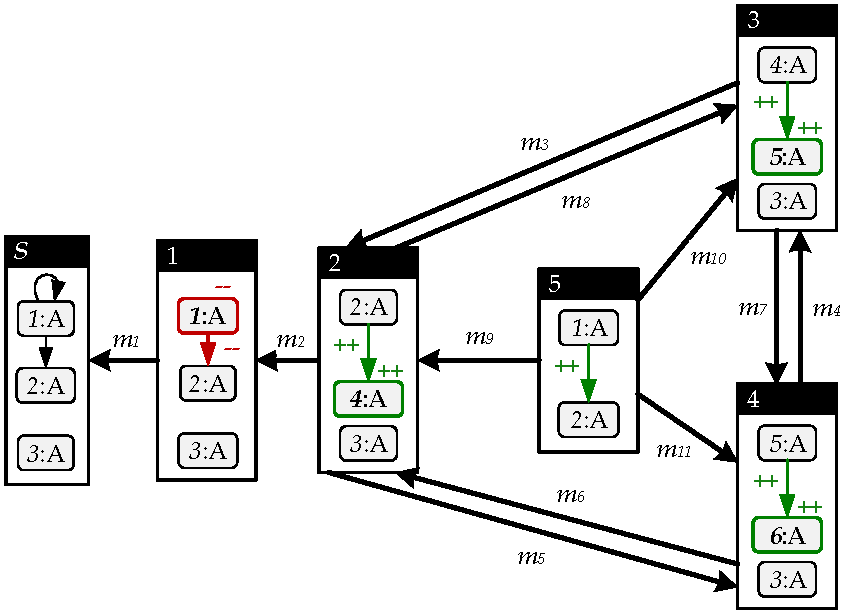
\includegraphics[width=.7\textwidth]{img/software_trans/graph_schema2.pdf}
\begin{math}
m_1=(1 \mapsto 1,2 \mapsto 2, 3 \mapsto 3);m_2=(2 \mapsto 2,3 \mapsto 3);m_3=(3 \mapsto 3, 4 \mapsto 4);m_4=(3 \mapsto 3, 5 \mapsto 5);m_5=(3 \mapsto 3, 2 \mapsto 6);m_6=(3 \mapsto 3,5 \mapsto 4);m_7=(3 \mapsto 3, 4 \mapsto 6);m_8=(2 \mapsto 5,3 \mapsto 3);m_9=(1 \mapsto 4,2 \mapsto 3);m_{10}=(1 \mapsto 5,2 \mapsto 3);m_{11}=(1 \mapsto 6,2 \mapsto 3)
\end{math}
\newline
\begin{math}
t_\GS(m_1)=S;s_\GS(m_1)=t_\GS(m_2)=\code{1};s_\GS(m_2)=s_\GS(m_5)=s_\GS(m_8)=t_\GS(m_3)=t_\GS(m_6)=t_\GS(m_9)=\code{2};s_\GS(m_3)=s_\GS(m_7)=t_\GS(m_4)=t_\GS(m_8)=t_\GS(m_{10})=\code{3};s_\GS(m_4)=s_\GS(m_6)=t_\GS(m_5)=t_\GS(m_7)=t_\GS(m_{11})=\code{4};s_\GS(m_9)=s_\GS(m_{10})=s_\GS(m_{11})=\code{5}
\end{math}
\end{center}
\caption{Recursive Graph Schema with Interweaving Cyclic Match-Paths}
\label{fig:sec-compl-software-trans:rec_graph_schema2}
\end{figure}

Finally, the semantics of a recursive graph schema is given by its graph language over the set of terminating recursive transformation sequences starting at start graph $S$.
Note that for some recursive graph schemata there may not exist a terminating recursive transformation sequence or a recursive transformation sequence at all and therefore, its language may be empty.
For example, the recursive graph schema in \cref{fig:sec-compl-software-trans:rec_graph_schema2} without rule \code{5} and adjacent matches $m_9$ to $m_{11}$ has no terminating match-path and therefore, no terminating recursive transformation sequence.
Moreover, for the complete schema in \cref{fig:sec-compl-software-trans:rec_graph_schema2} there exists an infinite set of terminating match-paths but all existing match-paths do not lead to a recursive transformation sequence due to violations of the gluing condition at the first match $m_1$ in each match-path.
The deletion of node \code{1:A} by applying rule \code{1} via match $m_1$ would result in a dangling reflexive edge on \code{1:A}.
Thus, in general, for a match-path there may not exists a corresponding recursive transformation sequence due to a violation of the gluing condition.

\begin{definition}[Graph Language of Recursive Graph Schemata]
\label{def:sec-compl-software-trans:lang_rec}
Let $\GS=((S,P),M,s_\GS,t_\GS)$ be a recursive graph schema.
The \emph{language $\Lang(\GS)$ of $\GS$}\index{recursive graph schema!language} is given by $\Lang(\GS):=\quotient{R(\GS)}{\sim}$ with $\quotient{R(\GS)}{\sim}$ being the quotient set of $R(\GS)$ by $\sim$, $R(\GS):=\{\der(t) \mid t\colon S \Trans{*}_\GS G, t \text{ is terminating}, t \text{ starts in }S\}$ being the set of all derived spans that are derivable by terminating recursive transformation sequences starting at start graph $S$ and $\sim$ being the equivalence relation on $R(\GS)$ where $g\colon S \to G \sim g'\colon S \to G'$ if and only if $G \cong G'$ with isomorphism $i\colon G \to G'$ and $i \circ g = g'$.
\envEndMarker
\end{definition}

\begin{remark}[Graph Language of Recursive Graph Schemata]
Note that $\sim$ is indeed an equivalence relation, i.e., 
\begin{enumerate*}
\item reflexivity: $g \sim g$ by isomorphism $i=\id_G\colon G \to G$ with $\id_G \circ g = g$,
\item symmetry: $g \sim g'$ if and only if $g' \sim g$ by inverse isomorphism $i^{-1}\colon G' \to G$ with $g=\id_G \circ g=i^{-1} \circ i \circ g\stackrel{\cref{def:sec-compl-software-trans:lang_rec}}{=} i^{-1} \circ g'$, and
\item transitivity: $g \sim g'$ and $g' \sim g''\colon S \to G''$ implies $g \sim g''$ by isomorphism $i' \circ i\colon G \to G''$ with isomorphism $i'\colon G' \to G''$ and $i' \circ i \circ g \stackrel{\cref{def:sec-compl-software-trans:lang_rec}}{=} i' \circ g' \stackrel{\cref{def:sec-compl-software-trans:lang_rec}}{=} g''$.
\end{enumerate*}
Moreover in $\M$-adhesive categories, $\paths=\paths'$ for $g=\der(t),g'=\der(t') \in R(\GS)$ with $t\colon S \Trans{path}_\GS G,t'\colon S \Trans{path'}_\GS G'$ implies $G \cong G'$ with isomorphism $i\colon G \to G'$ and $i \circ g = g'$ (thus, $g \sim g'$) by the uniqueness of pushout complements and pushout objects.
Furthermore, language $\Lang(\GS)$ may contain the same graph $G$ several times but each with different derived spans $\der(t_i)\colon S \to G$.
  \begin{center}
  \begin{tikzpicture}
  \node[inner sep=0pt] (a) at (0,0) {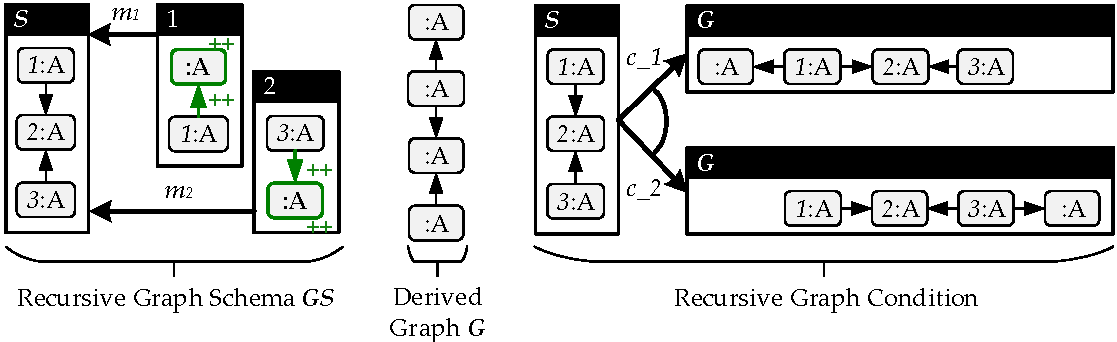
\includegraphics[width=.87\textwidth]{img/software_trans/graph_schema3.pdf}};
  \node[inner sep=0pt] (b) at (1.02,.55) {$\vee$};
  \end{tikzpicture}
  \end{center}
This is important in order to obtain recursive graph constraints over that language with the desired semantics.
For example, from the recursive graph schema $\GS$ from above, graph $G$ can be derived by two terminating recursive transformation sequences $t_1\colon S \Trans{(m_1)}_\GS G$ and $t_2\colon S \Trans{(m_2)}_\GS G$ starting at $S$, i.e., via the two match-paths $(m_1)$ and $(m_2)$, respectively.
The mappings along morphisms $m_1,m_2,c_1=\der(t_1)$ and $c_2=\der(t_2)$ are expressed by identifications of the numbers for each node.
Thus, $\Lang(\GS)=\{[c_1],[c_2]\}$ is given by two equivalence classes which contain one of the two derived spans to graph $G$, respectively, resulting in a recursive graph constraint $(\exists(S \trans{c_1} G,\true)) \vee (\exists(S \trans{c_2} G,\true))$ which disjoints both path-options.
Therefore, a graph $G'$ generally satisfies the constraint, if for all occurrences of pattern $S$ in $G'$
\begin{enumerate*}
\item[a)] either node \code{:A} is attached to the top node \code{1:A}, or
\item[b)] to the bottom node \code{3:A}.
\end{enumerate*}
\envEndMarker
\end{remark}

\begin{remark}[Graph Language of Recursive Graph Schemata]
Note that the language of a recursive graph schema may be empty if no terminating recursive transformations do exist: 
\begin{enumerate*}
\item either due to a violation of the gluing condition (cf. \cref{fig:sec-compl-software-trans:rec_graph_schema2}), or
\item no terminating match-paths do exist, or
\item the set of productions $P$ is empty.
\end{enumerate*}
This is true since an empty set $P$ implies that the set of matches $M$ is also empty and furthermore, the language is defined over recursive transformation sequences w.r.t. match paths and empty match paths (empty recursive transformation sequences) are not defined explicitly (cf. \cref{rem:sec-compl_software-trans:rec_trafo}).
\envEndMarker
\end{remark}

\begin{example}[Graph Language of Recursive Graph Schemata]
\label{ex:sec-compl-software-trans:lang_rec_schema}
For the recursive graph schema in \cref{ex:sec-compl-software-trans:rec_schema}, \cref{fig:sec-compl-software-trans:rec_graph_lang} illustrates all graphs that can be derived by terminating recursive transformation sequences with starting at start graph $S$.
This includes graph $G_0$ from below via recursive transformation $t_0\colon S \Trans{(m_1)}_\GS G_0$ and all graphs $G_1,G_2,G_3$ etc. that can be obtained from $G_0$ by arbitrarily adding a list of attribute (and class) nodes before $j$ (and after $i$) recursively via corresponding recursive transformations.
\begin{center}
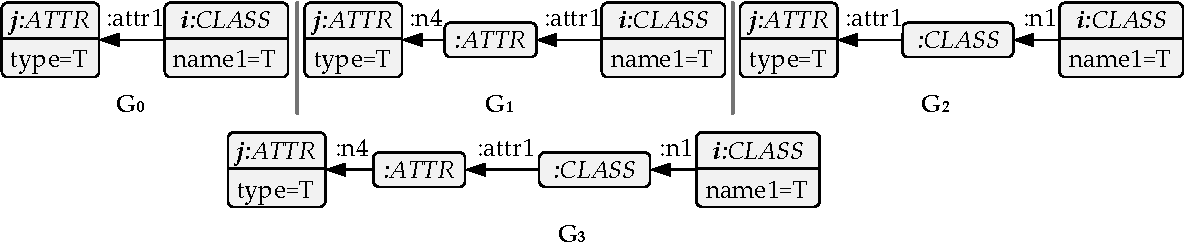
\includegraphics[width=.96\textwidth]{img/software_trans/graphs.pdf}
\end{center}
As the schema contains cyclic match-paths, its language is infinite containing equivalence class $[\der(t_0)\colon S \to G_0]$ and the infinite set of equivalence classes $[\der(t_i)\colon S \to G_i]$ of all other derived spans that can be obtained via terminating recursive transformations $t_i\colon S \Trans{*}_\GS G_i$ starting at $S$.
\envEndMarker
\end{example}

Based on the language of recursive graph schemata with start graph $S$ and productions $P$, we define recursive (infinite) graph conditions.
A recursive graph condition is defined by a disjunction over all derived spans of the language as mappings to the conclusion graphs with $S$ being the premise graph.
We assume a restriction of $P$ to productions that are non-deleting only in order to obtain an induced morphism as derived span for each pair of (premise,conclusion) graphs instead of spans of morphisms (cf. \cref{rem:sec-gc-gc:der_span_non_deleting}).

\begin{definition}[Recursive Graph Condition]
\label{def:sec-compl-software-trans:sem_rec_cond}
Let $\GS=((S,P),M,s_\GS,t_\GS)$ be a recursive graph schema with non-deleting productions $P$ and $\Lang(\GS)$ be the graph language of $\GS$.
The \emph{recursive graph condition $c_\GS$}\index{recursive graph condition} w.r.t. $\GS$ is defined by $c_\GS=\vee_{[\ac] \in \Lang(\GS)}\exists(\ac\colon S \to \_,\true)$.
\envEndMarker
\end{definition}

Recursive graph conditions are in $\M$-normal form which is necessary to be used in the verification of domain completeness in \cref{sec-dc-verification,thm:C-extensionCompleteness}.

\begin{proposition}[Recursive Graph Conditions in $\M$-normal form]
\label{prop:sec-compl-software-trans:rec_cond_constr_m_norm}
In $\M$-adhesive categories, \emph{each recursive graph condition is in $\M$-normal form}\index{recursive graph condition!$\M$-normal form}.
\envEndMarker
\end{proposition}

\begin{proof}
Technically, non-deleting productions $p=(L_p \transB{l_p} K_p \trans{r_p} R_p)$ are defined with $l_p=\id_{L_p}$ resulting in recursive transformation steps in \cref{def:sec-compl-software-trans:rec_trafo} with $l'_p \in \M$, $l'_p$ being an isomorphism, $l'^{-1}_p \in \M$ and $l'^{-1}_p$ being its inverse morphism for $\M$-adhesive categories.
This holds, since, the class $\M$ is closed under isomorphisms (therefore, $l_p \in \M$), iso- and $\M$-morphisms are closed under pushouts (therefore, $l'_p \in \M$ and $l'_p$ is isomorphism) and the inverse morphism $l'^{-1}_p$ is in $\M$ by $\M$-decomposition of $l'_p \circ l'^{-1}_p=\id_O \in \M$.
Furthermore, $r'_p \in \M$, since, $r_p \in \M$ by the definition of productions and $\M$-morphisms are closed under pushouts.
Thus, the induced morphisms $\ac$ in \cref{def:sec-compl-software-trans:sem_rec_cond} are in $\M$ by $\M$-composition of $r'_p \circ l'^{-1}_p$, i.e., recursive graph conditions are in $\M$-normal form.
\end{proof}

Note that recursive graph conditions are standard nested conditions and therefore, the standard logical operations for forming bigger conditions can be applied, e.g., negation, con- and dis-junction with other conditions.
Especially the possibility to negate recursive conditions not only allows the definition of graph constraints of the form ``For all $S$ there exists some regular path" and ``there exists $S$ with some regular path" but also ``For all $S$ there does not exist some regular path'' and ``there exists $S$ without some regular path''.

\begin{remark}[Conjunctive Recursive Graph Conditions]
Note that recursive graph conditions are explicitly defined by a disjunction over the conclusions that is infinite for infinite sets of conclusions.
A corresponding notion where the disjunction is replaced by a conjunction would disagree with the intrinsic idea of having an option of (infinite) conclusions.
Moreover, a conjunction over an infinite set of recursively growing conclusions as constraint can only be satisfied by infinite graphs. 
\envEndMarker
\end{remark}

\begin{example}[Recursive Graph Constraint]
\label{ex:sec-compl-software-trans:rec_cond}
For the recursive graph schema in \cref{ex:sec-compl-software-trans:rec_schema}, the corresponding infinite recursive graph constraint is generally satisfied by a graph $G$, if in $G$ for all attributes $A$ of type $T$ there is a class $C_1$ with name $T$ defined, and $A$ is the attribute of some class $C_2$ and either $C_1=C_2$ or $C_1$ is defined before $C_2$.
The membership of an attribute to a class is expressed by paths of \code{:attr1} and \code{:n4} edges between both.
The fact that a class is defined before some other class is expressed by paths of \code{:n1} edges between both.
\envEndMarker
\end{example}

In \cite{DBLP:conf/rta/BertrandDKSS12}, the decidability of reachability and coverability in various types of graph transformation systems with different restrictions were investigated.
In the following, we investigate the decidability of partial reachability in graph grammars and recursive graph schemata in order to conclude over the decidability of the satisfaction of recursive graph conditions in \cref{thm:sec-compl-software-trans:sat_rec_cond}.
In contrast to reachability, given a graph $G$, partial reachability of $G$ requires that there is at least one transformation sequence to some $G'$ such that there is an $\M$-morphism from $G'$ to $G$ instead of an isomorphism between both.
Conversely, coverability requires that there is at least one transformation sequence to some $G'$ such that there is an $\M$-morphism from $G$ to $G'$.
Thus, partial reachability is the inverse of coverability w.r.t. reachability.

While for finite-state graph transformation systems, the partial reachability problem is obviously decidable by iterating over all states and check partial reachability for each, it is different for infinite-state graph transformation systems (states are graphs and transitions between states are transformation steps).
We use infinite-state graph transformation systems for specifying infinite graph languages of recursive graph patterns.
While graph grammars with deleting rules can be used for specifying such languages where the start graph is the base case of the recursion and further graph patterns are obtained by recursively deleting and adding elements, the partial reachability problem is undecidable for general graph grammars by a reduction from the halting problem over turing machines (cf. \cref{prop:sec-compl-software-trans:dec_part_reach,item:sec-compl-software-trans:dec_part_reach2}).
However, for recursive graph schemata (with deleting rules), it turns out to be decidable by their monotone nature which is given by the restrictions for matches, since,
\begin{enumerate*}
\item matches are pre-defined, and
\item each recursive transformation step in a recursive transformation uses the co-match of the previous step to further restrict the match
\end{enumerate*} (cf. \cref{prop:sec-compl-software-trans:dec_part_reach,item:sec-compl-software-trans:dec_part_reach3}).
This leads to the decidability of the satisfaction of recursive graph conditions in \cref{thm:sec-compl-software-trans:sat_rec_cond}.

\begin{definition}[Partial Reachability Problem]
Let $G$ be a graph, $\GG=(S,P)$ be a graph grammar with start graph $S$ and a set of productions $P$ and $\GS=(\GG,M,s_\GS,t_\GS)$ be a recursive graph schema.
The \emph{partial reachability problem}\index{partial reachability!problem} for graph grammars (recursive graph schemata) is defined as follow: Is there a (terminating recursive) transformation sequence $S \Trans{*} G'$ ($S \Trans{*}_\GS G'$) that starts in $S$ to some graph $G'$ via productions $P$ (in $\GS$) such that there exists an $\M$-morphism $m\colon G' \to G,m \in \M$?
\envEndMarker
\end{definition}

% \begin{definition}[Monotone Graph Grammar]
% Let $<$ be a strict partial order over the set of graphs where $G < G'$ if and only if graph $G$ has fewer structural graph elements than $G'$.
% \emph{A graph grammar $\GG=(P,S)$ with productions $P$ and start graph $S$ is monotone} if for each transformation step $G \Trans{p \in P} G'$ with existing sequence $S \Trans{*} G$ via $P$ it holds that $G < G'$.
% \envEndMarker
% \end{definition}
% 
% Obviously, each typed attributed graph grammar $\GG=(P,S)$ with productions $P$ of the form $p\colon L \transB{l} K \trans{r} R,l,r \in \M$ and transformation steps based on the double pushout approach is monotone if $L < R$ for each production $p \in P$.
% In the following, we consider typed attributed graph grammars with non-deleting productions $p\colon L \to R \in \M$ only ($K=L$) and furthermore, $L < R$.
% Thus, each production of the grammar is non-trivial in the sense that it creates at least one graph element.

\begin{proposition}[Decidability of Partial Reachability]
\label{prop:sec-compl-software-trans:dec_part_reach}
\index{partial reachability!decidability}Let $G$ be a graph, $\GG=(S,P)$ be a graph grammar with start graph $S$ and a set of productions $P$ and $\GS=(\GG,M,s_\GS,t_\GS)$ be a recursive graph schema.
\begin{enumerate}
  \item For grammars $\GG$ with non-deleting productions $P$ only and finite graphs $G$, the (partial) reachability problem is decidable in $\M$-adhesive categories. 
  \item \label{item:sec-compl-software-trans:dec_part_reach2}In general and in particular for grammars $\GG$ with finite sets of productions $P$ and finite graphs $G$ in the $\M$-adhesive category $(\cat{Graphs}_\TG,\M)$ of typed graphs with(out) application conditions (and $\M$-matches), the (partial) reachability problem is undecidable.
  \item \label{item:sec-compl-software-trans:dec_part_reach3}In $(\cat{\AGraphs_\ATGI},\M)$, for recursive graph schemata $\GS$ with a finite set of matches $M$ and finite graphs $G$, the (partial) reachability problem is decidable.\envEndMarker
\end{enumerate}
\end{proposition}

\begin{proof}
The proof is presented in \cref{sec-proofs:prop:sec-compl-software-trans:dec_part_reach}.
\end{proof}

\begin{theorem}[Decidability of Satisfaction of Recursive Graph Conditions]
\label{thm:sec-compl-software-trans:sat_rec_cond}
\index{recursive graph condition!satisfaction!decidability}Let $\GS=((S,P),M,s_\GS,t_\GS)$ be a recursive graph schema with a finite set of matches $M$, $p\colon S \to G$ be a morphism ($G$ be a finite graph) and $c_\GS$ be the recursive graph condition w.r.t. $\GS$.
Then, \emph{the problem whether $p$ ($G$) satisfies $c_\GS$ is decidable in $\cat(\AGraphs_\ATGI,\M)$}.
\envEndMarker
\end{theorem}

\begin{proof}
By \cref{def:condition-satisfaction,def:sec-compl-software-trans:sem_rec_cond}, $p \models c_\GS=\vee_{[\der(t)] \in \Lang(\GS)}\exists(\der(t)\colon S \to \_,\true)$ if and only if $\exists [\der(t)\colon S \to G'] \in \Lang(\GS).p \models \exists(\der(t),\true) \Leftrightarrow \exists$ terminating recursive transformation $t$ in $\GS$ that starts in $S$ with $\der(t)\colon S \to G'$ and $p \models \exists(\der(t),\true) \Leftrightarrow\exists$ terminating recursive transformation $t\colon S \Trans{*}_\GS G'$ in $\GS$ that starts in $S$ such that there exists $q\colon G' \to G \in \M$ with $q \circ \der(t)=p$ which is decidable by \cref{prop:sec-compl-software-trans:dec_part_reach,item:sec-compl-software-trans:dec_part_reach3} by checking the commuting property for all existing $q \in \M$ which also terminates with the procedure from the proof of \cref{prop:sec-compl-software-trans:dec_part_reach,item:sec-compl-software-trans:dec_part_reach3} for finite $G$.
For recursive graph constraints $c_\GS$ over $S$, listing all occurrences of $S$ in $G$ (all $p\colon S \to G \in \M$) also terminates and results in a finite set for finite $G$.
For each occurrence of $S$ in $G$ we can proceed with $c_\GS$ as given above.
\end{proof}

Recursive structures in recursive conditions are expressed by cycles of matches $M$ in the underlying recursive graph schema.
Thus, a recursive graph schema with cycles in $M$ may lead to an infinite recursive graph constraint which is constructed step-wise by pumping the underlying condition via the repeated iteration of cycles.
The verification procedure of domain completeness terminates for finite graph constraints only.
Therefore, we present two techniques for deriving finite constraints from infinite recursive graph constraints by making them tighter or weaker.
The idea behind tightened recursive graph conditions is to omit all conclusion graphs from an infinite recursive condition $c_\GS$ that exceed a specific upper bound.
The upper bound is defined by a dedicated graph $G_u$ and the tightened condition of $c_\GS$ is formed over all conclusion graphs of $c_\GS$ with inclusions to $G_u$ only.
Therefore, the set of graphs satisfying a set of tightened constraints is a subset of the set of graphs satisfying the set of the corresponding originial infinite constraints but not necessarily vice versa.
However, it holds that a successful verification of domain completeness w.r.t. the tightened constraints and a given TGG implies that all graphs up to the upper bound satisfying the original infinite constraints can be completely transformed via the TGG.
In contrast to that, the idea behind weakened recursive graph conditions is to list for each acyclic, terminating recursive transformation sequence $S \Trans{\paths}_\GS G$ over $\GS$ and for all match-cycles in $\GS$ that are reachable from match-path $\paths$ all relevant overlappings of a single iteration of each cycle and $G$ as conclusion graphs.
Therefore, the derived conditions cover those graph structures only that may occur when iterating each cycle the last time by omitting those structures that are created by the iterations in between.
For positive recursive constraints $c_\GS$, the set of graphs satisfying the corresponding weakened constraint is a superset of the set of graphs satisfying $c_\GS$.
Thus, a successful verification of domain completeness w.r.t. weakened constraints and a given TGG implies domain completeness w.r.t. the original (infinite) constraints $c_\GS$ and TGG which implies furthermore that all graphs satisfying constraints $c_\GS$ can be completely transformed via the TGG.

\begin{definition}[Tightened Graph Language of Recursive Graph Schemata]
\label{def:sec-dc-general-rec:t_g_lang}
Let $\GS=((S,P),M,s_\GS,t_\GS)$ be a recursive graph schema.
Let $\Lang(\GS)$ be the graph language of $\GS$ and graph $G_u$ be an upper bound.
The \emph{tightened language $\Lang_t(\GS,G_u) \subseteq \Lang(\GS)$}\index{recursive graph schema!language!tightened} of $\GS$ and w.r.t. $G_u$ is given by $\Lang_t(\GS,G_u):=\{[\ac] \mid [\ac\colon S \to G] \in \Lang(\GS),\exists i\colon G \to G_u \in \M\}$.
\envEndMarker
\end{definition}

Before defining weakened conditions, we define the notions of $\M$-decomposition, initial $\M$-subobject and weakened language of recursive graph schemata at first.
An $\M$-decomposition of a morphism $\tr\colon A \to B$ is a decomposition of $\tr$ into two morphisms $\tr_1\colon A \to C,\tr_2\colon C\to B$ where both $\tr_1$ and $\tr_2$ are in $\M$.
For example in $(\cat{\Graphs},\M)$, $\M$-decompositions are a restriction of general decompositions of morphisms in the sense that graph $A$ is guaranteed to be a sub-graph of $C$ and $C$ is a sub-graph of $B$ whereas in general decompositions $C$ may be ``bigger'' than $B$ with an non-injective morphism $\tr_2$.
Similar to the concept of an $\M$-initial object which is considered as the ``smallest'' $\M$-subobject of all objects of a category, we introduce the weaker notion of an initial $\M$-subobject which is only the ``smallest" $\M$-subobject concerning one object of a category, respectively.
While a category may not have an $\M$-initial object, it may have an initial $\M$-subobject for each object.
 
\begin{definition}[$\M$-decomposition of Morphisms]
\emph{An $\M$-decomposition $d$ of an $\M$-morphism $\tr\colon L \to R$}\index{$\M$-decomposition of morphisms}, in short $\tr$-$\M$-decomposition, consists of two $\M$-morphisms $d=(L \trans{\tr_1} L' \trans{\tr_2} R)$ with $\tr_2 \circ \tr_1 = \tr$ and $\tr_1, \tr_2 \in \M$.
\envEndMarker
\end{definition}

\begin{definition}[Initial $\M$-subobject]
\label{def:sec-compl-software-trans:in_M_subobj}
Given an $\M$-adhesive category $(\cat{C},\M)$ and an object $G \in \cat{C}$.
Then, \emph{$\M$-subobject $[i_G\colon I_G \to G \in \M]$ of $G$ is initial}\index{$\M$-subobject!initial}, if for each $\M$-subobject $[a\colon A \to G \in \M]$ of $G$ there exists an (unique) $\M$-morphism $i_A\colon I_G \to A \in \M$ with $a \circ i_A = i_G$.
An $\M$-adhesive category $(\cat{C},\M)$ has initial $\M$-subobjects, if for each object $G \in \cat{C}$ there exists an initial $\M$-subobject.
\envEndMarker
\end{definition}

\begin{remark}[Initial $\M$-subobject]
\label{rem:sec-compl-software-trans:in_M_subobj}
Note that the uniqueness of morphism $i_A$ is optional as it follows directly from $a \in \M$ with $\M$ being a class of monomorphisms, since, $i_{A,1},i_{A,2} \in \M$ with $a \circ i_{A,1}=i_G=a \circ i_{A,2}$ implies that $i_{A,1}=i_{A,2}$.
\envEndMarker
\end{remark}

Initial $\M$-subobjects can be constructed by the extremal $\E$-$\M$-factorisation of initial morphisms.
Furthermore, initial $\M$-subobjects are unique up to isomorphism.

\begin{proposition}[Construction \& Uniqueness of Initial $\M$-subobjects]
\label{prop:sec-compl-software-trans:constr_uniqu_init_msubobj}
Given an $\M$-adhesive category $(\cat{C},\M)$ with an extremal $\E$-$\M$-factorisation and initial object $I$.
Then, \emph{the initial $\M$-subobject $[i_{G,2}\colon I_G \to G \in \M]$ for an object $G \in \cat{C}$ can be constructed}\index{$\M$-subobject!initial!construction} by the extremal $\E$-$\M$-factorisation $i_{G,2} \circ i_{G,1}=i_G$ of the initial morphism $i_G\colon I \to G$ with $i_{G,1}\colon I \to I_G \in \E,i_{G,2}\colon I_G \to G \in \M$.
Furthermore, in $\M$-adhesive categories, \emph{initial $\M$-subobjects are unique up to isomorphism}\index{$\M$-subobject!initial!uniqueness}.
\envEndMarker
\end{proposition}

\begin{proof}
We have to show that $\M$-subobject $[i_{G,2}\colon I_G \to G \in \M]$ of $G$ is initial.
\begin{center}
\begin{tikzpicture}[]
\fill (0,0) node[inner sep=1pt] (I) {$I$};
\fill (0,0) node[below of=I,yshift=-.5cm,inner sep=1pt] (IG) {$I_G$};
\fill (0,0) node[below of=IG,yshift=-.5cm,inner sep=1pt] (G) {$G$};
\fill (0,0) node[left of=IG,xshift=-2.5cm,inner sep=1pt] (A) {$A$};
\fill (0,0) node[right of=A,xshift=.75cm,yshift=.3cm,inner sep=1pt] (O) {$O$};
\fill (0,0) node[right of=IG,xshift=-.25cm,inner sep=1pt] (1) {$(=)$};
\fill (0,0) node[right of=O,xshift=.2cm,yshift=.3cm,inner sep=1pt] (2) {$(=)$};
\fill (0,0) node[left of=O,xshift=.5cm,yshift=.45cm,inner sep=1pt] (3) {$(=)$};
\fill (0,0) node[below of=O,inner sep=1pt] (4) {$(1)$};
%
\fill (0,0) node[right of=G,xshift=5cm,inner sep=1pt] (G2) {$\overline{G}$};
\fill (0,0) node[right of=IG,xshift=3cm,inner sep=1pt] (IG1) {$\overline{I}_{G,1}$};
\fill (0,0) node[right of=IG,xshift=7cm,inner sep=1pt] (IG2) {$\overline{I}_{G,2}$};
\fill (0,0) node[right of=I,xshift=5cm,inner sep=1pt] (O2) {$\overline{O}$};
\fill (0,0) node[above of=G2,yshift=.25cm,inner sep=1pt] (5) {$(2)$};
%
{
\pgfsetarrows{right hook-latex}
\path (A) edge[bend right=30] node[fill=white]{\scriptsize{$a$}} (G);
\path (O) edge[] node[above]{\scriptsize{$o_2$}} (IG);
\path (IG1) edge[] node[fill=white]{\scriptsize{$\overline{i}_{G,1}$}} (G2);
\path (O2) edge[] node[fill=white]{\scriptsize{$o_2$}} (IG2);
\path (IG1) edge[dotted,bend right=35] node[fill=white]{\scriptsize{$o'_1$}} (O2);
%
\pgfsetarrows{left hook-latex}
\path (O) edge[] node[above]{\scriptsize{$o_1$}} (A);
\path (IG) edge[] node[right]{\scriptsize{$i_{G,2}$}} (G);
\path (IG) edge[bend left=35,dotted] node[below]{\scriptsize{$o_2^{-1}$}} (O);
\path (IG2) edge[] node[fill=white]{\scriptsize{$\overline{i}_{G,2}$}} (G2);
\path (O2) edge[] node[fill=white]{\scriptsize{$o_1$}} (IG1);
\path (IG2) edge[dotted,bend left=35] node[fill=white]{\scriptsize{$o'_2$}} (O2);
%
\pgfsetarrows{-latex}
\path (I) edge[in=0,out=0,looseness=1.5] node[fill=white]{\scriptsize{$i_G$}} (G);
\path (I) edge[in=90,out=180] node[fill=white]{\scriptsize{$i_A$}} (A);
\path (I) edge[dotted] node[fill=white]{\scriptsize{$i_O$}} (O);
%
\pgfsetarrows{->>}
\path (I) edge[] node[right]{\scriptsize{$i_{G,1}$}} (IG);
}
\end{tikzpicture}
\end{center}
Let $[a\colon A \to G \in \M]$ be an $\M$-subobject of $G$ and $i_A\colon I \to A$ be the initial morphism to $A$.
We construct pullback $(1)$ $(o_1,o_2)$ over morphisms $(a,i_{G,2})$.
By $\M$-morphisms are closed under pullbacks, $o_1,o_2 \in \M$.
By the uniqueness of the initial morphism, $i_G=i_{G,2} \circ i_{G,1}=a \circ i_A$.
Thus, by the universal property of pullbacks, there exists a unique morphism $i_O\colon I \to O$ with $o_1 \circ i_O=i_A$ and $o_2 \circ i_O=i_{G,1}$.
By the definition of class $\E$ with $i_{G,1} \in \E$ and $o_2 \in \M$, $o_2$ is an isomorphism with inverse isomorphism $o_2^{-1} \in \M$ and $o_2 \circ o_2^{-1} = \id_{I_G}$ $^{(*^1)}$, since, class $\M$ is closed under isomorphisms.
By $\M$-composition, $o_1 \circ o_2^{-1} \in \M$, $o_1 \circ o_2^{-1}$ is unique by \cref{rem:sec-compl-software-trans:in_M_subobj} and furthermore, $a \circ o_1 \circ o_2^{-1} \stackrel{(1)}{=} i_{G,2} \circ o_2 \circ o_2^{-1} \stackrel{(*^1)}{=} i_{G,2} \circ \id_{I_G} = i_{G,2}$.
The resulting initial $\M$-subobjects of the presented construction are unique, since, extremal $\E$-$\M$-factorisations are unique up to isomorphism in the given $\M$-adhesive category.
In general, apart from the construction, the uniqueness of initial $\M$-subobjects in $\M$-adhesive categories is shown as follows.
Given two initial $\M$-subobjects $[\overline{i}_{G,1}\colon \overline{I}_{G,1} \to \overline{G} \in \M]$ and $[\overline{i}_{G,2}\colon \overline{I}_{G,2} \to \overline{G} \in \M]$ of $\overline{G}$.
We construct pullback $(2)$ $(o_1,o_2)$ over $(\overline{i}_{G,1},\overline{i}_{G,2})$ with $o_1,o_2 \in \M$, since, $\M$-morphisms are closed under pullbacks and furthermore, $\overline{i}_{G,1} \circ o_1,\overline{i}_{G,2} \circ o_2\in \M$ by $\M$-composition.
By \cref{def:sec-compl-software-trans:in_M_subobj}, there exists $o'_2\colon \overline{I}_{G,2} \to \overline{O} \in \M$ with $\overline{i}_{G,1} \circ o_1 \circ o'_2=\overline{i}_{G,2}$ $^{(*^1)}$.
Analogously, there exists $o'_1\colon \overline{I}_{G,1} \to \overline{O} \in \M$ with $\overline{i}_{G,1} \circ \id_{\overline{I}_{G,1}} = \overline{i}_{G,1} = \overline{i}_{G,2} \circ o_2 \circ o'_1 \stackrel{(*^1)}{=} \overline{i}_{G,1} \circ o_1 \circ o'_2 \circ o_2 \circ o'_1$.
By $\overline{i}_{G,1} \in \M$ and $\M$ being a class of monomorphisms, $o_1 \circ o'_2 \circ o_2 \circ o'_1=\id_{\overline{I}_{G,1}}$.
Conversely, $\overline{i}_{G,2} \circ \id_{\overline{I}_{G,2}} = \overline{i}_{G,2} \stackrel{(*^1)}{=} \overline{i}_{G,1} \circ o_1 \circ o'_2 = \overline{i}_{G,2} \circ o_2 \circ o'_1 \circ o_1 \circ o'_2$.
By $\overline{i}_{G,2} \in \M$ being a monomorphism, $o_2 \circ o'_1 \circ o_1 \circ o'_2 = \id_{\overline{I}_{G,2}}$.
Thus, $o_2 \circ o'_1$ is an isomorphism with commuting $(2)$.
\end{proof}

\begin{example}[Initial $\M$-subobject]
The category $(\cat{\AGraphs_\ATGI},\M)$ has $(\varnothing,T_\DSIG)$ as initial object with $\varnothing$ being the empty graph except for the data nodes and $T_\DSIG$ being the term algebra of data signature $\DSIG$.
The initial $\M$-subobject of an object $(G,D) \in \cat{\AGraphs_\ATGI}$ is constructed by the extremal $\E$-$\M$-factorisation of the initial morphism $i_G\colon (\varnothing,T_\DSIG) \to (G,D)$.
Thus, the initial $\M$-subobject of $(G,D)$ with $\DSIG$-algebra $D$ is $[i'_G\colon (\varnothing,D) \to (G,D) \in \M]$ with $\varnothing$ being the empty graph except for the data nodes and $i'_G=(i'_{G,G},i'_{G,D})$ being the empty morphism $i'_{G,G}\colon \varnothing \to G$ on the graph part and identity $i'_{G,D}=\id_D\colon D \to D$ on the data part.
Note that, $(\cat{\AGraphs_\ATGI},\M)$ has an initial object but no $\M$-initial object, since, $\M$-morphisms are isomorphisms on the data part and this does not hold for all initial morphisms in $(\cat{\AGraphs_\ATGI},\M)$.
\envEndMarker
\end{example}

The result in \cref{prop:sec-compl-software-trans:init_M_subobj_along_M} we use to prove the well-definedness of the construction of weakened languages of recursive graph schemata in \cref{prop:sec-compl-software-trans:weakened_lang_well_def}.

\begin{proposition}[Initial $\M$-subobjects along $\M$-Morphisms]
\label{prop:sec-compl-software-trans:init_M_subobj_along_M}
In an $\M$-adhesive category with initial $\M$-subobjects, let $a\colon A \to B \in \M$ be an $\M$-morphism and $[i_A\colon I_A \to A \in \M]$ be the initial $\M$-subobject of $A$.
Then, \emph{$[a \circ i_A\colon I_A \to B]$ is the initial $\M$-subobject of $B$}\index{$\M$-subobject!initial!along $\M$}.
\envEndMarker
\end{proposition}

\begin{proof}
By $\M$-composition $a \circ i_A \in \M$, i.e., $[a \circ i_A \in \M]$ is an $\M$-subobject of $B$.
Let $[i_B\colon I_B \to B \in \M]$ be the initial $\M$-subobject of $B$.
Then, there exists an unique morphism $i_{I_A}\colon I_B \to I_A \in \M$ with $a \circ i_A \circ i_{I_A}=i_B$ $^{(*^1)}$.
By $\M$-composition, $[i_A \circ i_{I_A} \in \M]$ is an $\M$-subobject of $A$.
Thus from $i_A$ being the initial $\M$-subobject of $A$ by assumption, there is $i_{I_B}\colon I_A \to I_B \in \M$ with $i_A \circ i_{I_A} \circ i_{I_B}=i_A=i_A \circ \id_{I_A} \stackrel{i_A\text{ is Mono}}{\Rightarrow} i_{I_A} \circ i_{I_B}=\id_{I_A}$ $^{(*^2)}$.
Moreover, $i_B \circ i_{I_B}\stackrel{(*^1)}{=}a \circ i_A \circ i_{I_A} \circ i_{I_B} \stackrel{(*^2)}{=} a \circ i_A$ $\Rightarrow i_B \circ i_{I_B} \circ i_{I_A}=a \circ i_A \circ i_{I_A} \stackrel{(*^1)}{=} i_B=i_B \circ \id_{I_B}$ $\stackrel{i_B\text{ is Mono}}{\Rightarrow} i_{I_B} \circ i_{I_A}=\id_{I_B}$ $^{(*^3)}$.
\begin{center}
\begin{tikzpicture}[]
\fill (0,0) node[inner sep=1pt] (IB) {$I_B$};
\fill (0,0) node[below of=IB,yshift=-.5cm,inner sep=1pt] (IA) {$I_A$};
\fill (0,0) node[right of=IA,xshift=1cm,inner sep=1pt] (A) {$A$};
\fill (0,0) node[right of=A,xshift=1cm,inner sep=1pt] (B) {$B$};
%
\fill (0,0) node[right of=IA,xshift=.5cm,yshift=.5cm,inner sep=1pt] (1) {$(1)$};
%
{
\pgfsetarrows{right hook-latex}
\path (IB) edge[] node[fill=white]{\scriptsize{$i_B$}} (B);
\path (IA) edge[] node[fill=white]{\scriptsize{$i_A$}} (A);
\path (A) edge[] node[fill=white]{\scriptsize{$a$}} (B);
\path (IB) edge[dotted, bend left=45] node[fill=white]{\scriptsize{$i_{I_A}$}} (IA);
\path (IA) edge[dotted, bend left=45] node[fill=white]{\scriptsize{$i_{I_B}$}} (IB);
%
\pgfsetarrows{left hook-latex}
%
\pgfsetarrows{-latex}
%
\pgfsetarrows{->>}
%
}
\end{tikzpicture}
\end{center}
By $(*^1),(*^2)$ and $(*^3)$, $i_{I_A}$ is an isomorphism with $(1)$ commutes and therefore, $[i_B]=[a \circ i_A]$.
\end{proof}

For the construction of weakened graph languages, we restrict productions to be non-deleting in order to avoid conflicts with violations of the gluing condition and introduce the equivalence of match-cycles (cf. \cref{rem:sec-compl-software-trans:con_weakened_lang}).
We are confident that the construction can be extended to general productions by integrating gluing condition checks.

\begin{definition}[Equivalence of Match-Cycles]
\label{def:sec-dc-general-rec:equ_match_cycles}
Let $\gg((m_i)_{i \in \{1\ldots n\}}):=\{(m_i,m_{i+1}) \mid 1 \leq i < n\} \cup \{(m_n,m_1)\}$ be an order over the matches of a given match-cycle $(m_i)_{i \in \{1\ldots n\}}$.
\emph{Two match-cycles $\paths_1$ and $\paths_2$ are equal up to shifting of matches}\index{match-path!match-cycle!equivalence up to shifting of matches} if and only if $\gg(\paths_1)=\gg(\paths_2)$.
Let $\GS$ be a recursive graph schema and $\paths$ be a match-cycle in $\GS$.
With $\gg_\GS(\paths):=\{\paths' \mid \text{$\paths'$ is match-cycle in $\GS$},\gg(\paths)=\gg(\paths')\}$ we denote the set of all match-cycles in $\GS$ that are equal to $\paths$ up to shifting of matches.
For match-paths $\paths$ in $\GS$ that are no match-cycles, we define $\gg_\GS(\paths):= \varnothing$.
Let $\Paths_{\_,\_}(\GS)$ be the set of all acyclic match-cycles in $\GS$ and $\sim$ be the equivalence relation on $\Paths_{\_,\_}(\GS)$ where $\paths_1 \sim \paths_2$ if and only if $\gg_\GS(\paths_1)=\gg_\GS(\paths_2)$.
With $\quotient{\Paths_{\_,\_}(\GS)}{\sim}$ we denote the equivalence classes of all acyclic match-cycles in $\GS$ that are equal up to shifting of matches.
\envEndMarker
\end{definition}

\begin{example}[Equivalence of Match-Cycles]
For the match-cycle $\paths=(m_7,m_8,m_6)$ in \cref{fig:sec-compl-software-trans:rec_graph_schema2}, $\gg_\GS(\paths)=\{(m_7,m_8,m_6),(m_6,m_7,m_8),(m_8,m_6,m_7)\}$.
\envEndMarker
\end{example}

\begin{definition}[Weakened Graph Language of Recursive Graph Schemata]
\label{def:sec-compl-software-trans:weakened_lang}
Let $\GS=((S,P),M,s_\GS,t_\GS)$ be a recursive graph schema with non-deleting productions $P$.
The \emph{weakened language $\Lang_w(\GS):=\quotient{\underline{\Lang}_w(\GS)}{\sim}$ of $\GS$}\index{recursive graph schema!language!weakened} is given by the quotient set of $\underline{\Lang}_w(\GS)$ by $\sim$ with $\sim$ being the equivalence relation from \cref{def:sec-compl-software-trans:lang_rec} and projection $\underline{\Lang}_w(\GS):=\{\ac \mid (\ac,n) \in \cup_{m \in \underline{\Paths}_S(\GS)}(\underline{\Lang}_w(m,1,\id_S,\id_S,1))\}$ with $\underline{\Paths}_S(\GS) \subseteq \Paths_S(\GS)$ being the set of all acyclic and terminating match-paths in $\GS$ that start in $S$ with construction $\underline{\Lang}_w$ as given inductively below.
\envEndMarker
\end{definition}

\begin{paragraph}{Construction}
\begin{center}
	$\underline{\Lang}_w((m_i)_{i \in \{1\ldots j\}},i,\ac,n,k)=\begin{cases}
	\cup_{(t,n') \in \mathcal{B}}(\underline{\Lang}_w((m_i)_{i \in \{1\ldots j\}}, i+1, & \text{, for } \ac\colon \_ \to A \text{ and}\\
	\der(t)\circ \ac,n',1)) \text{ with } \mathcal{B}= & \text{if } i \leq j \text{ and }\\
	\{(t,n') \mid t\colon A \Trans{(s_\GS(m_i),m_i,n)}_{\GS,n'} B\} & (\Pset = \varnothing \text{ or } k=2)\\
	\cup_{(\ac',n') \in \mathcal{C}}(\underline{\Lang}_w((m_i)_{i \in \{1\ldots j\}},i, & \text{, for } \ac\colon \_ \to A \text{ and}\\
	\ac',n',2)) \text{ with } \mathcal{C}=\{(\ac,n)\} \cup & \text{if } i \leq j \text{ and }\\
	\cup_{\paths \in \Pset}(A \oplus B_\paths) \text{ where } & \Pset \neq \varnothing\\
	B_\paths=\underline{\Lang}_w(\paths,1,\id_R,\id_R,2) \text{ for} & \\
	\paths=(m'_k)_{k \in \{1\ldots l\}} \text{ and } m'_1\colon L \to R & \\
	\{(\ac,n)\} & \text{, otherwise}\\
	\end{cases}$
\end{center}
with switch $k \in \{1,2\}$, $\overline{\Pset}=\Paths_{t_\GS(m_i),t_\GS(m_i)}(\GS) \setminus \gg_\GS((m_i)_{i \in \{1\ldots j\}})$ being the set of all match-cycles in $\GS$ that start and end in $t_\GS(m_i)$ except all paths that are equal up to shifting to the path that is currently being handled, $\Pset \subseteq \overline{\Pset}$ being all paths in $\overline{\Pset}$ that are acyclic and $\oplus$ defined as follows:
$A \oplus B_\paths:=\cup_{d \in \mathcal{D}}(\{(a'_2 \circ \ac,a'_1 \circ \overline{n}') \mid \cond\})$ where in contrast to $(\ac,n) \in \mathcal{C}$ which represents the case with no iterations of cycles via match-path $\paths \in \Pset$, $A \oplus B_\paths$ represents arbitrary iterations by forming all relevant overlappings of the result of a single iteration $\iter \in B_\paths$ and $A$ where:
\begin{center}
\begin{tikzpicture}[]
\fill (0,0) node[inner sep=1pt] (I) {$I_L$};
\fill (0,0) node[right of=I,xshift=1cm,inner sep=1pt] (I') {$I'_{L}$};
\fill (0,0) node[right of=I',xshift=1cm,inner sep=1pt] (Lk') {$L$};
\fill (0,0) node[right of=Lk',xshift=4cm,inner sep=1pt] (Gk) {$L'$};
\fill (0,0) node[below of=Lk',yshift=-.5cm,inner sep=1pt] (R) {$R$};
\fill (0,0) node[below of=R,yshift=-.5cm,inner sep=1pt] (G2) {$R$};
\fill (0,0) node[below of=G2,yshift=0cm,inner sep=1pt] (G) {$A$};
\fill (0,0) node[right of=Lk',xshift=3cm,inner sep=1pt] (O) {$O$};
\fill (0,0) node[right of=G2,xshift=3cm,inner sep=1pt] (G'') {$R''$};
\fill (0,0) node[right of=G,xshift=4cm,inner sep=1pt] (G') {$A'$};
%
\fill (0,0) node[right of=R,xshift=.25cm,yshift=1cm,inner sep=1pt] (4) {$(2)$};
\fill (0,0) node[right of=R,xshift=2cm,yshift=0cm,inner sep=1pt] (5) {$(3)$};
\fill (0,0) node[right of=G2,xshift=.25cm,yshift=.5cm,inner sep=1pt] (6) {$(4)$};
\fill (0,0) node[right of=R,xshift=3.5cm,yshift=0cm,inner sep=1pt] (7) {$(5)$};
%
\fill (0,0) node[left of=I,xshift=-1cm,inner sep=1pt] (R3) {$R$};
\fill (0,0) node[below of=R3,xshift=-2cm,yshift=-.5cm,inner sep=1pt] (L2) {$L$};
\fill (0,0) node[right of=L2,xshift=1cm,inner sep=1pt] (L'2) {$L'$};
\fill (0,0) node[below of=L2,xshift=0cm,yshift=-.5cm,inner sep=1pt] (R2) {$R$};
\fill (0,0) node[right of=R2,xshift=1cm,inner sep=1pt] (R'2) {$R'$};
%
\fill (0,0) node[right of=L2,xshift=0cm,yshift=-.75cm,inner sep=1pt] (8) {$(PO)$};
\fill (0,0) node[right of=L'2,xshift=-.5cm,inner sep=1pt] (9) {$(=)$};
%
{
\pgfsetarrows{right hook-latex}
\path (I) edge[] node[fill=white]{\scriptsize{$i_{L,1}$}} (I');
\path (I') edge[] node[fill=white]{\scriptsize{$i_{L,2}$}} (Lk');
\path (Lk') edge[bend left=25] node[fill=white]{\scriptsize{$\overline{\ac}'$}} (Gk);
\path (I') edge[bend right=45] node[fill=white]{\scriptsize{$m$}} (R);
\path (Lk') edge[dotted] node[fill=white]{\scriptsize{$o$}} (O);
\path (R) edge[dotted] node[fill=white]{\scriptsize{$o'$}} (O);
\path (G2) edge[dotted] node[fill=white]{\scriptsize{$\der(t)$}} (G'');
\path (G) edge[bend right=25,dotted] node[fill=white]{\scriptsize{$a'_2$}} (G');
%
\path (R2) edge[] node[fill=white]{\scriptsize{$\overline{\ac}$}} (R'2);
\path (L2) edge[dotted] node[fill=white]{\scriptsize{$\overline{\ac}'$}} (L'2);
%
\pgfsetarrows{left hook-latex}
\path (Lk') edge[] node[fill=white]{\scriptsize{$m'_1$}} (R);
\path (R) edge[] node[fill=white]{\scriptsize{$\id_R$}} (G2);
\path (G2) edge[] node[left]{\scriptsize{$n$}} (G);
\path (O) edge[dotted] node[fill=white]{\scriptsize{$a''$}} (G'');
\path (R) edge[dotted] node[fill=white]{\scriptsize{$n'$}} (G'');
\path (Gk) edge[dotted] node[fill=white]{\scriptsize{$a'_1$}} (G');
%
\path (L2) edge[] node[fill=white]{\scriptsize{$m'_1$}} (R2);
\path (L'2) edge[dotted] node[fill=white]{\scriptsize{$\overline{m}'_1$}} (R'2);
\path (R3) edge[bend left=75] node[fill=white]{\scriptsize{$\overline{n}$}} (R'2);
\path (R3) edge[dotted] node[fill=white]{\scriptsize{$\overline{n}'$}} (L'2);
%
\pgfsetarrows{-latex}
%
\pgfsetarrows{->>}
%
}
\end{tikzpicture}
\end{center}
\begin{enumerate}
  \item \label{item:sec-compl-software-trans:weakened_lang:1}$\mathcal{D}=\{d=(I_L \trans{i_{L,1}} I'_L \trans{i_{L,2}} L) \mid d \text{ is } i_L \text{-} \M \text{-decomposition for initial } \M \text{-subobject } [i_L\colon I_L \to L \in \M] \text{ of } L\}$, and
  \item $\cond$:
  \begin{enumerate}
    \item \label{item:sec-compl-software-trans:weakened_lang:2a}$\iter=(\overline{\ac}\colon R \to R',\overline{n}\colon R \to R') \in B_\paths$,
	\item \label{item:sec-compl-software-trans:weakened_lang:2b}$(a'_1\colon L' \to A',a'_2\colon A \to A')$ is pushout over $(\overline{\ac}' \circ i_{L,2},n \circ m)$,
    \item \label{item:sec-compl-software-trans:weakened_lang:2c}$(\overline{\ac}' \in \M,\overline{m}'_1 \in \M)$ is pushout complement over $(m'_1,\overline{\ac})$ resulting in pushout $(PO)$ with induced morphism $\overline{n}' \in \M$ and $\overline{m}'_1 \circ \overline{n}'=\overline{n}$, 
    \item \label{item:sec-compl-software-trans:weakened_lang:2e}$m\colon I'_L \to R \in \M$ such that $\exists t\colon R \Trans{p'}_{\GS,n'} R''$ with $p' \in \overline{\Pset}$ or $\der(t)=n'=\id_R$ such that
    \begin{enumerate*}
    \item \label{item:sec-compl-software-trans:weakened_lang:2e1}$\exists a''\colon O \to R'' \in \M$ for pushout $(o,o')$ over $(i_{L,2},m)$ with
    \item \label{item:sec-compl-software-trans:weakened_lang:2e2}$(2)+(3)$ commutes, and
    \item \label{item:sec-compl-software-trans:weakened_lang:2e3}$(3)+(4)$ commutes.\envEndMarker
    \end{enumerate*}   
  \end{enumerate}
\end{enumerate}
\end{paragraph}

\begin{remark}[Construction of Weakened Graph Languages]
\label{rem:sec-compl-software-trans:con_weakened_lang}
The construction is based on the idea that cyclic, terminating match-paths are obtained from acyclic, terminating paths by possibly pumping the path after each match by adding arbitrary match-cycles.
Therefore, the construction starts with an acyclic, terminating match-path $m$ in $\GS$ that starts in $S$, $\id_S$ for $\ac$ as derived span, $\id_S$ for $n$ as co-match and switch $k=1$.
The construction passes through $m$ step-wise with matches $m_i \in m$:
\begin{enumerate}
  \item \label{item:sec-compl-software-trans:cons_weakened_lan:1} If there is no match-cycle from and to the target $t_\GS(m_i)$ of $m_i$ which differs from all paths that are equal to the path that is currently being handled up to shifting of matches ($\mathcal{P}=\varnothing$) and that may lead to a cyclic match-path before $m_i$ or if switch $k=2$, then a recursive transformation step $t$ with co-match $n'$ is performed via production $s_\GS(m_i)$, match $m_i$ and co-match $n$.
  The construction recursively proceeds with the next match in $m$ for $m_i$, an extended derived span $\der(t) \circ \ac$ for $\ac$, co-match $n'$ for $n$ and switch $k=1$.
  \item If there is a match-cycle from and to $t_\GS(m_i)$ which differs from all paths that are equal to the path that is currently being handled up to shifting of matches ($\mathcal{P}\neq\varnothing$), then before performing the recursive transformation step via match $m_i$ in \cref{item:sec-compl-software-trans:cons_weakened_lan:1} with switch $k=2$, all cycles that may pump path $m$ before $m_i$ are considered at first.
  Therefore, for each $\paths$ in $\mathcal{P}$ representing a single cycle iteration before $m_i$, the construction is called recursively and the result $B_\paths$ is overlapped with the current result $A$ by $A \oplus B_\paths$.
  Beside the case $(\ac,n) \in \mathcal{C}$ where no cycles via $\paths$ are iterated, set $A \oplus B_\paths$ simulates arbitrary cycle iterations by relevant overlappings.
  The overlappings are formed by $\M$-decompositions $\mathcal{D}$ (cf. \cref{def:sec-compl-software-trans:weakened_lang,item:sec-compl-software-trans:weakened_lang:1}) and pushout constructions over common overlapping object $I'_L$ (cf. \cref{def:sec-compl-software-trans:weakened_lang,item:sec-compl-software-trans:weakened_lang:2b}).
  An overlapping is relevant, if the overlapping ``occurs'' in recursive transformations in $\GS$ (cf. \cref{prop:sec-compl-software-trans:weakened_lang_well_def,item:sec-compl-software-trans:well_def_con_w_lan:3}), i.e, the part which is added to $A$ by the overlapping is guaranteed to be added by some existing recursive transformation (cf. \cref{def:sec-compl-software-trans:weakened_lang,item:sec-compl-software-trans:weakened_lang:2e2}) in the given context (cf. \cref{def:sec-compl-software-trans:weakened_lang,item:sec-compl-software-trans:weakened_lang:2e3}).
\end{enumerate}
Thus, for acyclic, terminating recursive transformations $t\colon S \Trans{\paths}_\GS G$, if there does not exist match-cycles in $\GS$ that are reachable from match-path $\paths$, then the construction behaves equivalent to $t$.
Otherwise, if match-cycles in $\GS$ exist that are reachable from $\paths$, then the result of the single iteration of each cycle is overlapped with intermediate results of $t$, therefore, simulating the last single iteration of each cycle in all contexts that occur in existing recursive transformations based on $t$.
In order to ensure that only a single iteration of each cycle $c$ is considered in recursive calls of the construction while an infinite number of iterations exists, the construction neglects cycles that are equal to $c$ up to shifting of matches while passing step-wise through $c$.
Otherwise, for match-cycle $c=(m_1\ldots m_n)$ at match $m_2$, the construction would additionally consider cycle $(m_2\ldots m_n,m_1)$ resulting in a two-time iteration of $c$, etc..
\envEndMarker
\end{remark}

\begin{example}[Weakened Graph Language of Recursive Graph Schemata]
\label{ex:sec-dc-general-rec:weakened_graph_lang}
\cref{fig:sec-compl-software-trans:wglex} illustrates the weakened graph language of the recursive graph schema $\GS$ in \cref{fig:sec-compl-software-trans:rec_graph}.
The language consists of 16 equivalence classes of morphisms $[\ac_i\colon S \to G_i]_{i \in \{0\ldots 15\}}$ where the mapping $\ac_i$ of the \code{:ATTR} node in $S$ to $G_i$ is given by node name $1$ in \cref{fig:sec-compl-software-trans:wglex}, respectively.
While graphs $G_0,G_1,G_4$ and $G_7$ are obtained by the four existing acyclic, terminating match-paths in $\GS$ that start in $S$, the other graphs are obtained by additional relevant overlappings with results of single match-cycle iterations that together represent all the ``last'' cycle iterations in all contexts that occur in cyclic, terminating recursive transformations in $\GS$ that start in $S$.
In detail, $G_0,G_1,G_4$ and $G_7$ are obtained by stepping through acyclic paths $(m_1,m_9),(m_1,m_2,m_7),(m_1,m_5,m_8)$ and $(m_1,m_5,m_4,m_7)$, respectively.
In contrast, $G_2$ is obtained by path $(m_1,m_2)$ followed by an overlapping with the result of iterating cycle $(m_3)$ once and the succeeding path $(m_7)$.
The overlapping is given by match $m_3$ itself with $m=m'_1=m_3$ and $i_{L,2}=\id_L$ in \cref{def:sec-compl-software-trans:weakened_lang,item:sec-compl-software-trans:weakened_lang:1} and $\der(t)=n'=\id_R$ in \cref{def:sec-compl-software-trans:weakened_lang,item:sec-compl-software-trans:weakened_lang:2e}.
Thus, the overlapping is relevant in the sense that it does occur in the recursive transformation w.r.t. path $(m_1,m_2,m_3,m_7)$ leading to $G_2$, i.e., acyclic path $(m_1,m_2,m_7)$ is pumped to a cyclic path $(m_1,m_2,m_3,m_7)$ via additional cycle $(m_3)$.
Analogously to $G_2$, $G_3$ is obtained by $(m_1,m_2)$ followed by an overlapping via cycle $(m_3)$ and succeeding $(m_7)$.
However this time, the overlapping is not exactly given by match $m_3$ itself but by $m'_1=m_3$ in \cref{def:sec-compl-software-trans:weakened_lang,item:sec-compl-software-trans:weakened_lang:1} and furthermore for rule \code{3:addNextClass} as source and target of $m_3$: Graph $I'_L$ consists of node \code{1:ATTR} only and morphisms $m=i_{L,2}=(1 \mapsto 1)$.
Therefore, the overlapping is given by a gluing (pushout) of the graph parts of the graph after $(m_1,m_2)$ and the RHS of rule \code{3:addNextClass} via common node \code{1:ATTR}.
Note that, there is a recursive transformation $t$ in \cref{def:sec-compl-software-trans:weakened_lang,item:sec-compl-software-trans:weakened_lang:2e} via path $p'=(m_3)$ such that $a''$ exists and $(2)+(3)$ and $(3)+(4)$ commute.
Thus, the overlapping is relevant in the sense that it does occur in recursive transformations w.r.t. paths of the form $(m_1,m_2,m_3,\ldots,m_3,m_7)$, i.e., acyclic path $(m_1,m_2,m_7)$ is pumped to cyclic paths $(m_1,m_2,m_3,\ldots,m_3,m_7)$ by adding an arbitrary number of additional cycles $(m_3)$.
Four other overlappings via $m'_1=m_3$ and $i_L$-$\M$-decompositions in \cref{def:sec-compl-software-trans:weakened_lang,item:sec-compl-software-trans:weakened_lang:1} technically exist but all violate the conditions in \cref{def:sec-compl-software-trans:weakened_lang,item:sec-compl-software-trans:weakened_lang:2e} and therefore, they are not considered for language construction:
\begin{enumerate*}
\item We assume that morphism $i_{L,2}=\id_L$ and $m=(1 \mapsto 1,2 \mapsto 2)$.
There are morphisms $a''$ but without commuting $(2)+(3)$ and $(3)+(4)$.
\item The three remaining overlappings each add a second \code{:ATTR} node and therefore, in all three cases there does not exists an injective morphism $a'' \in \M$, since, production \code{3:addNextClass} does not create \code{:ATTR} nodes.
\envEndMarker
\end{enumerate*}
\begin{figure}[!tb]
\begin{center}
  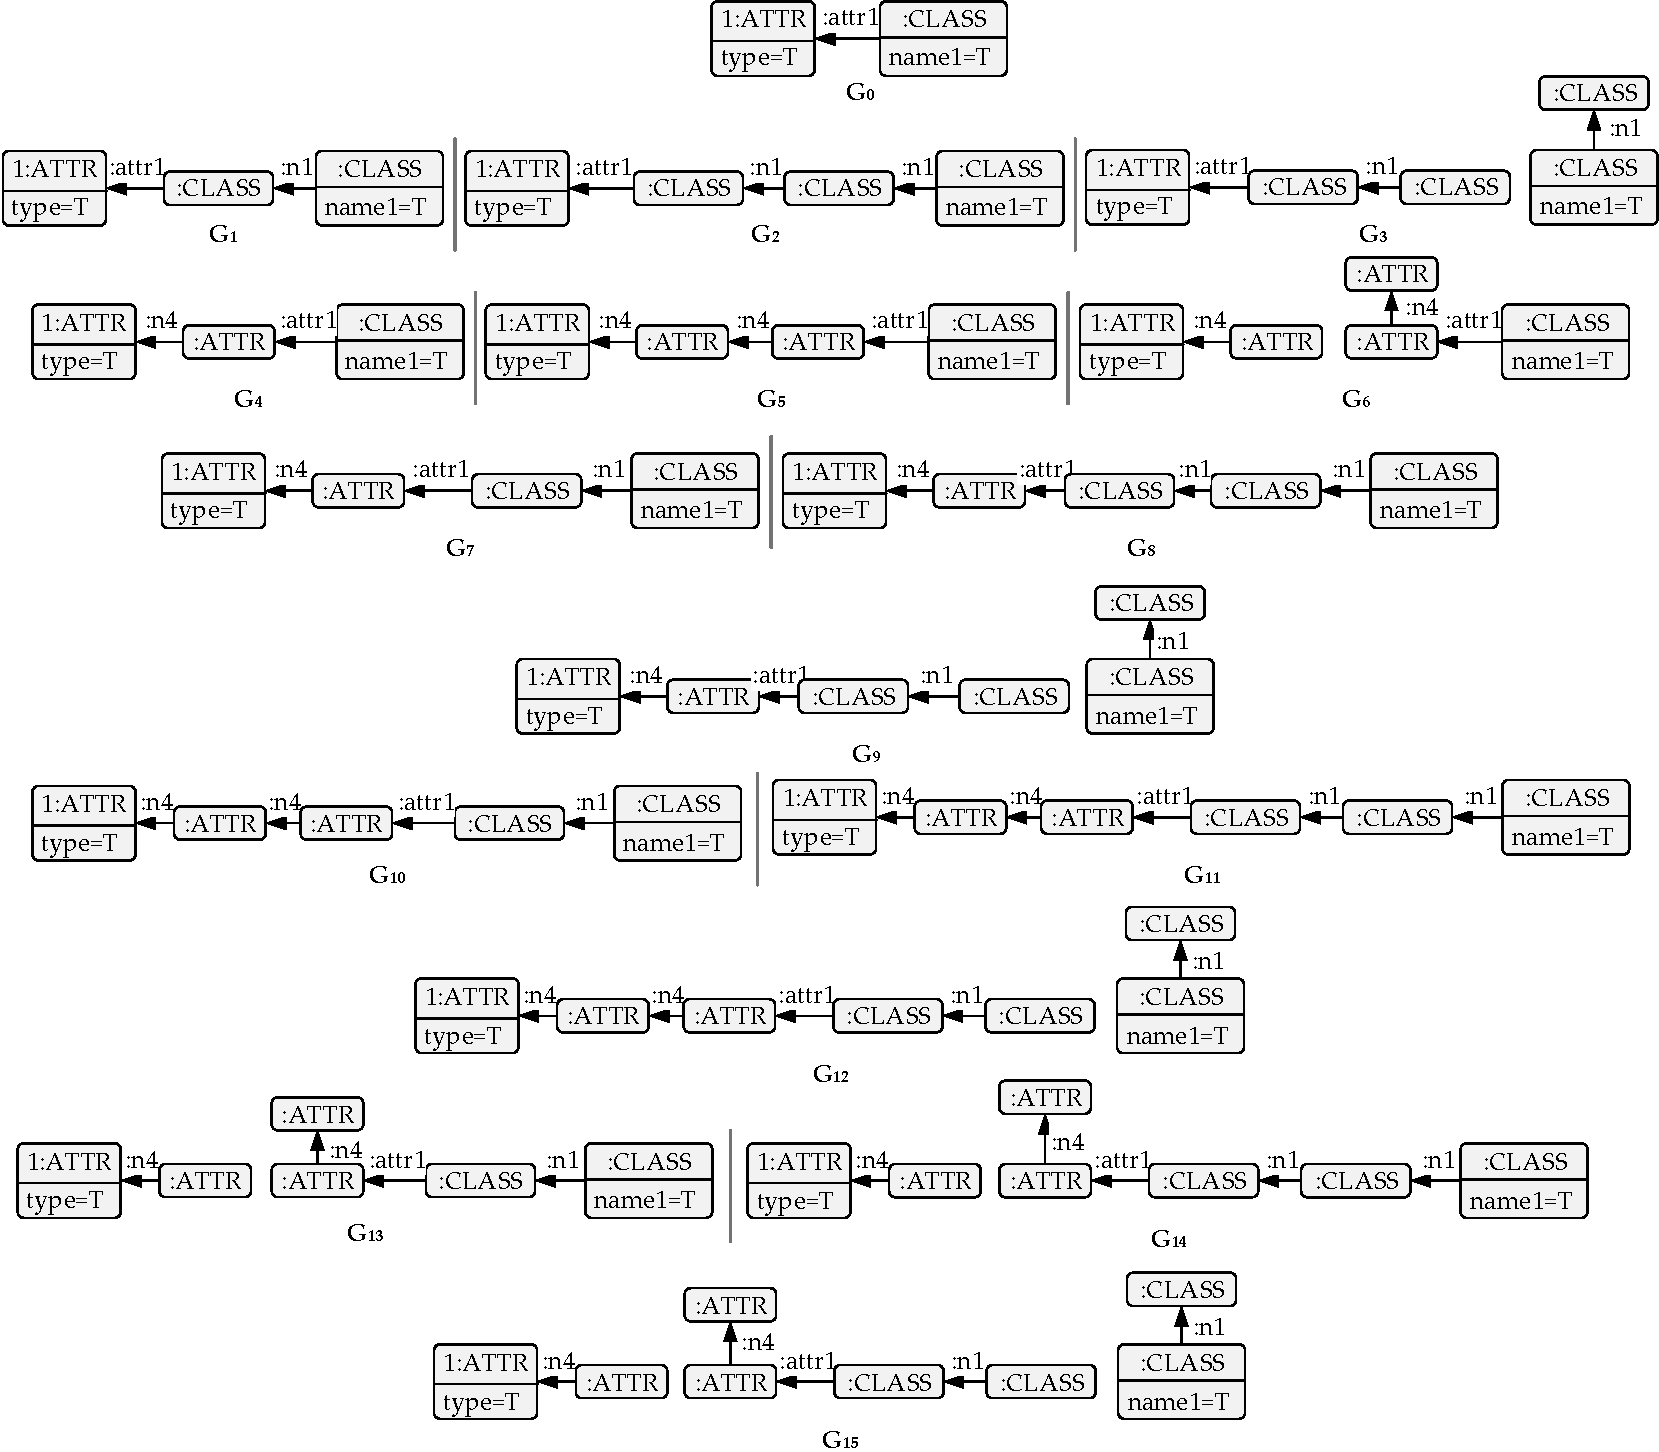
\includegraphics[width=\textwidth]{img/software_trans/wlex.pdf}
\end{center}
\caption{Weakened Graph Language}
\label{fig:sec-compl-software-trans:wglex}
\end{figure}
\end{example}

In the following, we show that the construction of weakened graph languages is well-defined in the sense that it leads to the desired set $\Lang_w(\GS)$ of equivalence classes of morphisms for a given recursive graph schema $\GS$ with start graph $S$.
In particular, 
\begin{enumerate*}
\item \label{item:sec-compl-software-trans:well_def:1}for each acyclic, terminating recursive transformation $t\colon S \Trans{*}_\GS G$ which starts in $S$, there is a class $[\der(t)] \in \Lang_w(\GS)$ that coincides with the derived span $\der(t)$ of $t$,
\item \label{item:sec-compl-software-trans:well_def:2}for each cyclic, terminating recursive transformation $t\colon S \Trans{*}_\GS G$ which starts in $S$, there is a class $[\ac] \in \Lang_w(\GS)$ that may not coincide with but partially reflect $\der(t)$, and
\item \label{item:sec-compl-software-trans:well_def:3}each $[\ac] \in \Lang_w(\GS)$ partially reflects the derived span $\der(t)$ of some terminating recursive transformation $t\colon S \Trans{*}_\GS G$ which starts in $S$.
\end{enumerate*}
We use \cref{item:sec-compl-software-trans:well_def:1,item:sec-compl-software-trans:well_def:2,item:sec-compl-software-trans:well_def:3} for showing that the language over general recursive graph constraints is a subset of the language over weakened recursive graph constraints in \cref{thm:sec-compl-software-trans:comp-lang-constraints} such that domain completeness w.r.t. weakened constraints implies domain completeness w.r.t. general constraints (cf. \cref{thm:sec-compl-software-trans:dom_compl_inf}).
Furthermore, \cref{item:sec-compl-software-trans:well_def:3} illustrates the fact that the weakened language contains (weakened constraints cover) correct cases only which increases the accuracy of the domain completeness verification w.r.t. weakened constraints by potentially omitting the verification of faulty cases.

\begin{proposition}[Well-Definedness of Construction of Weakened Graph Languages]
\label{prop:sec-compl-software-trans:weakened_lang_well_def}
Let $\GS=((S,P),M,s_\GS,t_\GS)$ be a recursive graph schema with non-deleting productions $P$, $\Lang(\GS)$ be the language of $\GS$ and $\Lang_w(\GS)$ be the weakened language of $\GS$.
For the construction of weakened graph languages, the following holds in $\M$-adhesive categories with effective pushouts and initial $\M$-subobjects:\index{recursive graph schema!language!well-definedness}
\begin{enumerate}
\item \label{item:sec-compl-software-trans:well_def_con_w_lan:1}For each terminating, acyclic $t\colon S \Trans{*}_\GS G$ which starts in $S$ there is $[\der(t)] \in \Lang_w(\GS)$,
\item \label{item:sec-compl-software-trans:well_def_con_w_lan:2}For each terminating, cyclic $t\colon S \Trans{*}_\GS G$ which starts in $S$ there is $[\ac\colon S \to G'] \in \Lang_w(\GS)$ such that there is an $\M$-morphism $i\colon G' \to G$ with $i \circ \ac=\der(t)$, and
\item \label{item:sec-compl-software-trans:well_def_con_w_lan:3}For each $[\ac\colon S \to G'] \in \Lang_w(\GS)$ there is terminating $t\colon S \Trans{*}_\GS G$ which starts in $S$ and $\M$-morphism $i\colon G' \to G$ such that $i \circ \ac=\der(t)$.\envEndMarker
\end{enumerate}
\end{proposition}

\begin{proof}
The proof is presented in \cref{sec-proofs:prop:sec-compl-software-trans:weakened_lang_well_def}.
\end{proof}

Based on the notions of tightened and weakened graph languages of recursive graph schemata, we define tightened and weakened recursive graph conditions according to \cref{def:sec-compl-software-trans:sem_rec_cond}.

\begin{definition}[Tightened \& Weakened Recursive Graph Condition]
\label{def:sec-dc-general-rec:t_w_g_constr}
Let $\GS$ be a recursive graph schema.
The recursive graph condition $c_\GS$ w.r.t. $\GS$ is \emph{(tightened w.r.t. a given upper bound $G_u$) weakened}\index{recursive graph condition!tightened}\index{recursive graph condition!weakened}, if it is formed over the (tightened) weakened graph language of $\GS$ (and w.r.t. $G_u$).
\envEndMarker
\end{definition}

\begin{example}[Tightened \& Weakened Recursive Graph Constraint]
The weakened recursive graph condition w.r.t. the recursive graph schema $\GS$ in \cref{ex:sec-compl-software-trans:rec_schema} is given by the disjunction over all morphisms of the corresponding weakened graph language of $\GS$ in \cref{ex:sec-dc-general-rec:weakened_graph_lang}.
Note that the weakened recursive graph constraint is only an approximation to the recursive graph constraint in \cref{ex:sec-compl-software-trans:rec_cond}.
More precisely, it is not required that for all attributes of type $T$ there is a class of name $T$ such that there is a path between both but the path may also be interrupted as illustrated by graphs $G_3,G_6,G_9,G_{12},G_{13},G_{14}$ and $G_{15}$ in \cref{fig:sec-compl-software-trans:wglex}.
In contrast to that, the tightened recursive graph constraint w.r.t. $\GS$ is equivalent to the recursive graph constraint in \cref{ex:sec-compl-software-trans:rec_cond} but only for graphs up to the given upper bound.
\envEndMarker
\end{example}

Analogously to \cref{prop:sec-compl-software-trans:rec_cond_constr_m_norm}, in the following we show that tightened and weakened recursive graph conditions are in $\M$-normal form which is necessary to be used in the verification of domain completeness in \cref{sec-dc-verification,thm:C-extensionCompleteness}.
Furthermore, we investigate the relationship between graph languages over recursive graph constraints in \cref{thm:sec-compl-software-trans:comp-lang-constraints} in order to conclude over the verification of domain completeness w.r.t. infinite graph constraints via \cref{sec-dc-verification,thm:C-extensionCompleteness} in \cref{thm:sec-compl-software-trans:dom_compl_inf}.
More precisely, the verification of domain completeness can be performed w.r.t. tightened \& weakened recursive graph constraints.
While for weakened recursive graph constraints we obtain a general result for domain completeness in \cref{thm:sec-compl-software-trans:dom_compl_inf,thm:sec-compl-software-trans:dom_compl_inf:2}, for tightened recursive graph constraints we obtain a result for domain completeness up to a given upper bound only in \cref{thm:sec-compl-software-trans:dom_compl_inf,thm:sec-compl-software-trans:dom_compl_inf:1}.

\begin{theorem}[Tightened \& Weakened Recursive Graph Conditions in $\M$-normal form]
\label{prop:sec-compl-software-trans:tight_weak_rec_cond_constr_m_norm}
In $\M$-adhesive categories with effective pushouts and initial $\M$-subobjects, \emph{each tightened \& weakened recursive graph condition is in $\M$-normal form}\index{recursive graph condition!tightened!$\M$-normal form}\index{recursive graph condition!weakened!$\M$-normal form}.
\envEndMarker
\end{theorem}

\begin{proof}
Let $\GS$ be a recursive graph schema, $c_\GS$ be the recursive graph condition, $c_{t,\GS}$ be the tightened recursive graph condition and $c_{w,\GS}$ be the weakened recursive graph condition w.r.t. $\GS$.
By \cref{def:sec-dc-general-rec:t_w_g_constr,def:sec-dc-general-rec:t_g_lang} it follows that $c_{t,\GS}$ is built up by a subset of morphisms of $c_\GS$.
Therefore by \cref{prop:sec-compl-software-trans:rec_cond_constr_m_norm} it follows that $c_{t,\GS}$ is in $\M$-normal form.
By \cref{prop:sec-compl-software-trans:weakened_lang_well_def,item:sec-compl-software-trans:well_def_con_w_lan:3}, for each morphism $\ac\colon S \to G'$ in $c_{w,\GS}$, there is a morphism $\der(t)\colon S \to G$ in $c_\GS$ (cf. \cref{def:sec-compl-software-trans:lang_rec,def:sec-compl-software-trans:sem_rec_cond}) and morphism $i \in \M$ such that $i \circ \ac=\der(t)$.
By \cref{prop:sec-compl-software-trans:rec_cond_constr_m_norm}, $\der(t) \in \M$ implying further that $\ac \in \M$ by $\M$-decomposition, i.e., $c_{w,\GS}$ is in $\M$-normal form.
\end{proof}

\begin{proposition}[Relationship between Languages over Recursive Graph Constraints]
\label{thm:sec-compl-software-trans:comp-lang-constraints}
Let $\GS$ be a recursive graph schema with non-deleting productions.
Furthermore, let $c_\GS$ be the recursive graph constraint, and $c_{w,\GS}$ be the weakened recursive graph constraint w.r.t. $\GS$.
Moreover, let $c_{t,\GS}$ be the tightened recursive graph constraint w.r.t. $\GS$ and upper bound $G_u$.
Then, the following holds in $\M$-adhesive categories with effective pushouts and initial $\M$-subobjects:
\begin{enumerate}
  \item $\Lang_I(\{c_\GS\})_{G_u} \subseteq \Lang_I(\{c_{t,\GS}\})$ and $\Lang_I(\{c_\GS\}) \subseteq \Lang_I(\{c_{w,\GS}\})$, and
  \item $\Lang(\{c_\GS\})_{G_u} \subseteq \Lang(\{c_{t,\GS}\})$ and $\Lang(\{c_\GS\}) \subseteq \Lang(\{c_{w,\GS}\})$
\end{enumerate}
where languages $\Lang_I(\{c_\GS\})_{G_u}$ and $\Lang(\{c_\GS\})_{G_u}$ are defined accordingly to \cref{sec-dc-verification,def:sec-dc-verification:dc_ub}.
\envEndMarker
\end{proposition}

\begin{proof}
Let $c_\GS,c_{t,\GS},c_{w,\GS}$ be the corresponding recursive graph constraints over $S$.

\noindent\textbf{Case ($c_{w,\GS}$)}: Let $G \in \Lang_I(\{c_\GS\})$ or $G \in \Lang(\{c_\GS\})$, respectively, and $p\colon S \to G \in \M$ be a corresponding morphism.
By \cref{sec-gt-gc,rem:sec-gc-gc:init_gen_sat} and \cref{sec-dc-general,def:sec-dc-general:lang}, $p \models c_\GS$ $\stackrel{\cref{sec-gt-gc,def:condition-satisfaction}}{\Leftrightarrow} \exists q\colon A \to G \in \M$ for some $\ac\colon S \to A$ in $c_\GS$ such that $q \circ \ac=p$ $\stackrel{\cref{def:sec-compl-software-trans:sem_rec_cond,def:sec-compl-software-trans:lang_rec}}{\Leftrightarrow} \exists q\colon A \to G \in \M$ for some $\der(t)=\ac\colon S \to A$ with $t\colon S \Trans{*}_\GS A$ being terminating and starting in $S$ such that $q \circ \der(t)=p$ $\stackrel{\cref{prop:sec-compl-software-trans:weakened_lang_well_def,item:sec-compl-software-trans:well_def_con_w_lan:1,item:sec-compl-software-trans:well_def_con_w_lan:2}\text{ and }\cref{def:sec-dc-general-rec:t_w_g_constr}}{\Rightarrow} \exists q\colon A \to G \in \M,\ac'\colon S \to A'$ in $c_{w,\GS}$, and $i\colon A' \to A \in \M$ such that $i \circ \ac'=\der(t)$ implying further that $\exists q \circ i\colon A' \to G \in \M$ for $\ac'\colon S \to A'$ in $c_{w,\GS}$ by $\M$-composition $\stackrel{\cref{sec-gt-gc,def:condition-satisfaction}}{\Leftrightarrow} p \models c_{w,\GS}$.
Therefore by \cref{sec-gt-gc,rem:sec-gc-gc:init_gen_sat}, $G \stackrel{I}{\models} c_{w,\GS}$ or $G \models c_{w,\GS}$, respectively, implying further that $G \in \Lang_I(\{c_{w,\GS}\})$ or $G \in \Lang(\{c_{w,\GS}\})$, respectively, by \cref{sec-dc-general,def:sec-dc-general:lang}.

\noindent\textbf{Case ($c_{t,\GS}$)}: Let $G \in \Lang_I(\{c_\GS\})_{G_u}$ or $G \in \Lang(\{c_\GS\})_{G_u}$, respectively, and $p\colon S \to G \in \M$ be a corresponding morphism.
By \cref{sec-dc-verification,def:sec-dc-verification:dc_ub}, $G \in \Lang_I(\{c_\GS\})$ or $G \in \Lang(\{c_\GS\})$, respectively, and furthermore, there is $i\colon G \to G_u \in \M$.
By \cref{sec-gt-gc,rem:sec-gc-gc:init_gen_sat} and \cref{sec-dc-general,def:sec-dc-general:lang}, $p \models c_\GS$ $\stackrel{\cref{sec-gt-gc,def:condition-satisfaction}}{\Leftrightarrow} \exists q\colon A \to G \in \M$ for some $\ac\colon S \to A$ in $c_\GS$ such that $q \circ \ac=p$.
Thus, by $\M$-composition there is $i \circ q\colon A \to G_u \in \M$ implying further that $\ac$ is a morphism in $c_{t,\GS}$ by \cref{def:sec-dc-general-rec:t_g_lang,def:sec-dc-general-rec:t_w_g_constr}, i.e., $p \models c_{t,\GS}$.
Therefore by \cref{sec-gt-gc,rem:sec-gc-gc:init_gen_sat}, $G \stackrel{I}{\models} c_{t,\GS}$ or $G \models c_{t,\GS}$, respectively, implying further that $G \in \Lang_I(\{c_{t,\GS}\})$ or $G \in \Lang(\{c_{t,\GS}\})$, respectively, by \cref{sec-dc-general,def:sec-dc-general:lang}.
\end{proof}

\begin{theorem}[Verification of Domain Completeness w.r.t. Recursive Graph Constraints]
\label{thm:sec-compl-software-trans:dom_compl_inf}
Let $\GG$ be a grammar, $\overline{\GS}$ be a set of recursive graph schemata with non-deleting productions, $C_{\overline{\GS}}$ be the set of recursive graph constraints, and $C_{w,\overline{\GS}}$ be the set of weakened recursive graph constraints w.r.t. $\overline{\GS}$.
Furthermore, let $C_{t,\overline{\GS}}$ be the set of tightened recursive graph constraints w.r.t. $\overline{\GS}$ and a common upper bound $G_u$.
Then, the following holds in $\M$-adhesive categories with effective pushouts and initial $\M$-subobjects for a given set of constraints $C$:
\begin{enumerate}
  \item \label{thm:sec-compl-software-trans:dom_compl_inf:1}$\Lang(C \cup C_{t,\overline{\GS}}) \subseteq \Lang(\GG)$ implies domain completeness up to upper bound $G_u$: $\Lang(C \cup C_{\overline{\GS}})_{G_u} \subseteq \Lang(\GG)$, and
  \item \label{thm:sec-compl-software-trans:dom_compl_inf:2}$\Lang(C \cup C_{w,\overline{\GS}}) \subseteq \Lang(\GG)$ implies domain completeness: $\Lang(C \cup C_{\overline{\GS}}) \subseteq \Lang(\GG)$.
  \envEndMarker
\end{enumerate}
\end{theorem}

\begin{proof}
\begin{enumerate}
  \item We assume $\Lang(C \cup C_{t,\overline{\GS}}) \subseteq \Lang(\GG)$.
  Let $G \in \Lang(C \cup C_{\ol{\GS}})_{G_u}$ with $C=C_I \cup C_G$ and $C_{\ol{\GS}}=C_{I,\ol{\GS}} \cup C_{G,\ol{\GS}}$ where constraints $C_I,C_{I,\ol{\GS}}$ are designated for initial satisfaction and $C_G,C_{G,\ol{\GS}}$ are designated for general satisfaction
  $\stackrel{\cref{sec-dc-verification,def:sec-dc-verification:dc_ub}}{\Leftrightarrow} G \in \Lang(C \cup C_{\ol{\GS}})$ and $\exists i\colon G \to G_u \in \M$
  $\stackrel{\cref{sec-dc-general,def:sec-dc-general:lang}}{\Leftrightarrow} G \in \Lang_I(C_I \cup C_{I,\ol{\GS}})$ and $G \in \Lang(C_G \cup C_{G,\ol{\GS}})$, i.e., $G \stackrel{I}{\models} C_I \cup C_{I,\ol{\GS}}$ and $G \models C_G \cup C_{G,\ol{\GS}}$ and $\exists i\colon G \to G_u \in \M$
  $\stackrel{\cref{sec-gt-gc,def:constr_sat}\text{ and }\cref{sec-dc-general,def:sec-dc-general:lang}}{\Rightarrow} G \in \Lang_I(C_I)$, $\forall c_\GS \in C_{I,\ol{\GS}}.G \in \Lang_I(\{c_\GS\})$ $,G \in \Lang(C_G)$, and $\forall c_\GS \in C_{G,\ol{\GS}}.G \in \Lang(\{c_\GS\})$ and $\exists i\colon G \to G_u \in \M$
  $\stackrel{\cref{sec-dc-verification,def:sec-dc-verification:dc_ub}}{\Rightarrow}$ $G \in \Lang_I(C_I)$, $\forall c_\GS \in C_{I,\ol{\GS}}.G \in \Lang_I(\{c_\GS\})_{G_u}$ $,G \in \Lang(C_G)$, and $\forall c_\GS \in C_{G,\ol{\GS}}.G \in \Lang(\{c_\GS\})_{G_u}$
  $\stackrel{\cref{thm:sec-compl-software-trans:comp-lang-constraints}}{\Rightarrow}$ $G \in \Lang_I(C_I)$, $\forall c_\GS \in C_{I,\ol{\GS}}.G \in \Lang_I(\{c_{t,\GS}\})$ $,G \in \Lang(C_G)$, and $\forall c_\GS \in C_{G,\ol{\GS}}.G \in \Lang(\{c_{t,\GS}\})$ with $c_{t,\GS} \in C_{t,\ol{\GS}}$
  $\stackrel{\cref{sec-gt-gc,def:constr_sat}\text{ and }\cref{sec-dc-general,def:sec-dc-general:lang}}{\Rightarrow}$ $G \in \Lang(C)$ and $G \in \Lang(C_{t,\ol{\GS}})$
  $\Rightarrow G \in \Lang(C \cup C_{t,\ol{\GS}})$
  $\stackrel{Assumption}{\Rightarrow}$ $G \in \Lang(\GG)$.
  \item We assume $\Lang(C \cup C_{w,\overline{\GS}}) \subseteq \Lang(\GG)$.
  Let $G \in \Lang(C \cup C_{\ol{\GS}})$ with $C=C_I \cup C_G$ and $C_{\ol{\GS}}=C_{I,\ol{\GS}} \cup C_{G,\ol{\GS}}$ where constraints $C_I,C_{I,\ol{\GS}}$ are designated for initial satisfaction and $C_G,C_{G,\ol{\GS}}$ are designated for general satisfaction
  $\stackrel{\cref{sec-dc-general,def:sec-dc-general:lang}}{\Leftrightarrow} G \in \Lang_I(C_I \cup C_{I,\ol{\GS}})$ and $G \in \Lang(C_G \cup C_{G,\ol{\GS}})$, i.e., $G \stackrel{I}{\models} C_I \cup C_{I,\ol{\GS}}$ and $G \models C_G \cup C_{G,\ol{\GS}}$
  $\stackrel{\cref{sec-gt-gc,def:constr_sat}\text{ and }\cref{sec-dc-general,def:sec-dc-general:lang}}{\Rightarrow} G \in \Lang_I(C_I)$, $\forall c_\GS \in C_{I,\ol{\GS}}.G \in \Lang_I(\{c_\GS\})$ $,G \in \Lang(C_G)$, and $\forall c_\GS \in C_{G,\ol{\GS}}.G \in \Lang(\{c_\GS\})$
  $\stackrel{\cref{thm:sec-compl-software-trans:comp-lang-constraints}}{\Rightarrow}$ $G \in \Lang_I(C_I)$, $\forall c_\GS \in C_{I,\ol{\GS}}.G \in \Lang_I(\{c_{w,\GS}\})$ $,G \in \Lang(C_G)$, and $\forall c_\GS \in C_{G,\ol{\GS}}.G \in \Lang(\{c_{w,\GS}\})$ with $c_{w,\GS} \in C_{w,\ol{\GS}}$
  $\stackrel{\cref{sec-gt-gc,def:constr_sat}\text{ and }\cref{sec-dc-general,def:sec-dc-general:lang}}{\Rightarrow}$ $G \in \Lang(C)$ and $G \in \Lang(C_{w,\ol{\GS}})$
  $\Rightarrow G \in \Lang(C \cup C_{w,\ol{\GS}})$
  $\stackrel{Assumption}{\Rightarrow}$ $G \in \Lang(\GG)$.
\end{enumerate}
\end{proof}

Finally, we show that tightened and weakened recursive graph constraints can effectively be used for verifying domain completeness.
This means that the constraints are actually finite under certain conditions such that the verification terminates (cf. \cref{th:sec-dc-verification:term_dc,thm:sec-compl-software-trans:fin_rec_gc}).
Note that the number of nestings of recursive graph constraints is finite by constructions \cref{def:sec-compl-software-trans:sem_rec_cond,def:sec-dc-general-rec:t_w_g_constr}.
For ensuring the finiteness of weakened recursive graph constraints, we introduce the notion of simple recursive graph schemata in \cref{def:sec-dc-general-rec:simple_rec_gr_schema}.
A recursive graph schema is simple if all acyclic match-cycles that are not equal up to shifting of matches are linked via at most one production as depicted in \cref{fig:sec-dc-general-rec:simple_rec_schema} (a).
The schemata in \cref{fig:sec-dc-general-rec:simple_rec_schema} (b) and (c) are not simple.
\cref{fig:sec-dc-general-rec:simple_rec_schema} (b) contains two acyclic match-cycles \code{(1)} and \code{(2)} that are linked via two productions.
\cref{fig:sec-dc-general-rec:simple_rec_schema} (c) contains a cycle of acyclic match-cycles \code{(1)}, \code{(2)} and \code{(3)} that are linked to each other via one production, respectively.
However, this situation always leads to an acyclic match-cycle \code{(4)} which is linked to other match-cycles via more than one production. 
Therefore, a cycle of acyclic match-cycles is also forbidden for simple recursive graph schemata.

\begin{figure}[!tb]
\begin{center}
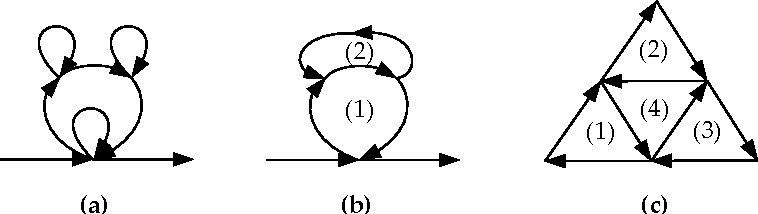
\includegraphics[width=.75\textwidth]{img/software_trans/simple.pdf}
\end{center}
\caption{Simple Recursive Graph Schema}
\label{fig:sec-dc-general-rec:simple_rec_schema}
\end{figure}

\begin{definition}[Simple Recursive Graph Schema]
\label{def:sec-dc-general-rec:simple_rec_gr_schema}
\index{recursive graph schema!simple}
Let $\GS$ be a recursive graph schema and $\quotient{\Paths_{\_,\_}(\GS)}{\sim}$ be the equivalence classes of all acyclic match-cycles in $\GS$ that are equal up to shifting of matches as defined in \cref{def:sec-dc-general-rec:equ_match_cycles}.
Then $\GS$ is simple, if for all $[\paths_1],[\paths_2] \in \quotient{\Paths_{\_,\_}(\GS)}{\sim}$ and for all $m_i,m_{i'} \in \paths_1$ and $m_j,m_{j'} \in \paths_2$ it holds that $s_\GS(m_i)=s_\GS(m_j)$ and $s_\GS(m_{i'})=s_\GS(m_{j'})$ implies that $m_i=m_{i'}$ and $m_j=m_{j'}$.
\envEndMarker
\end{definition}

\begin{example}[Simple Recursive Graph Schema]
The recursive graph schema in \cref{fig:sec-compl-software-trans:rec_graph} is simple while the schema in \cref{fig:sec-compl-software-trans:rec_graph_schema2} is not simple.
\envEndMarker
\end{example}

\begin{theorem}[Finiteness of Recursive Graph Constraints]
\label{thm:sec-compl-software-trans:fin_rec_gc}
Let $\GS=((S,P),M,s_\GS,t_\GS)$ be a recursive graph schema.
\begin{enumerate}
  \item The recursive graph constraint $c_\GS$ w.r.t. $\GS$ is finite, if:
  \begin{enumerate}
    \item \label{thm:sec-compl-software-trans:fin_rec_gc:1}The set $\Paths_S(\GS)$ of acyclic, terminating match-paths in $\GS$ that start in $S$ is finite, and 
    \item \label{thm:sec-compl-software-trans:fin_rec_gc:2}For all match-paths $\paths \in \Paths_S(\GS)$ there is no match-cycles in $\GS$ that is reachable from $\paths$.
  \end{enumerate}
  \item In $(\AGraphs_\ATGI,\M)$, the tightened recursive graph constraint $c_{t,\GS}$ w.r.t. $\GS$ and upper bound $G_u$ is finite, if:
  \begin{enumerate}
    \item \label{thm:sec-compl-software-trans:fin_rec_gc:5}Recursive graph schema $\GS$ contains non-deleting productions $P$ only,
    \item \label{thm:sec-compl-software-trans:fin_rec_gc:3}Graph $G_u$ is finite, and
    \item \label{thm:sec-compl-software-trans:fin_rec_gc:4}The set of matches $M$ is finite.
  \end{enumerate}
  \item In $(\AGraphs_{\ATGI,\fin},\M_\fin)$, the weakened recursive graph constraint $c_{w,\GS}$ w.r.t. $\GS$ is finite, if:
  \begin{enumerate}
    \item \label{thm:sec-compl-software-trans:fin_rec_gc:6}The set of matches $M$ is finite, and
    \item \label{thm:sec-compl-software-trans:fin_rec_gc:7}Recursive graph schema $\GS$ is simple.
    \envEndMarker
  \end{enumerate}
\end{enumerate}
\end{theorem}

\begin{proof}
By \cref{sec-gt-gc,def:condition-satisfaction}, for constraint $c$ is finite we have to show that the index set $I$ of every disjunction $\vee_{i \in I}$ in $c$ is finite.
\begin{enumerate}
  \item By assumptions \cref{thm:sec-compl-software-trans:fin_rec_gc,thm:sec-compl-software-trans:fin_rec_gc:1,thm:sec-compl-software-trans:fin_rec_gc:2} and \cref{def:sec-compl-software-trans:lang_rec}, language $\Lang(\GS)$ of $\GS$ is the finite set of derived spans of the finite set of terminating recursive transformation sequences starting at $S$.
  Thus, by construction \cref{def:sec-compl-software-trans:sem_rec_cond}, $c_\GS$ is finite.
  \item W.l.o.g. and by assumption \cref{thm:sec-compl-software-trans:fin_rec_gc,thm:sec-compl-software-trans:fin_rec_gc:5} we assume that each recursive transformation step via a production $p \in P$ and match $m \in M$ creates at least one graph element while preserving the remaining elements.
  By $M$ being finite by assumption \cref{thm:sec-compl-software-trans:fin_rec_gc,thm:sec-compl-software-trans:fin_rec_gc:4}, we have finitely many possibilities at each step to continue with the next step until we have exceeded finite upper bound $G_u$ (cf. assumption \cref{thm:sec-compl-software-trans:fin_rec_gc,thm:sec-compl-software-trans:fin_rec_gc:3}).
  Therefore, there are finitely many recursive transformation sequences up to upper bound $G_u$ leading to finitely many derived spans in tightened language $\Lang_t(\GS,G_u)$ of $\GS$ and w.r.t. $G_u$ (cf. \cref{def:sec-dc-general-rec:t_g_lang}).
  Thus, by construction \cref{def:sec-dc-general-rec:t_w_g_constr}, $c_{t,\GS}$ is finite.
  \item We focus on the construction of weakened languages in \cref{def:sec-compl-software-trans:weakened_lang}.
  There are at most $|M|!$ acyclic match-paths in $\GS$, each consisting of at most $|M|$ matches, since, having a match $m \in M$ two-times in a path yields a cyclic path.
  Therefore by assumption \cref{thm:sec-compl-software-trans:fin_rec_gc,thm:sec-compl-software-trans:fin_rec_gc:6} of $M$ being finite, the set of acyclic match-paths in $\GS$ is finite and furthermore, each acyclic match-path consists of a finite set of matches.
  Thus, the set $\underline{\Paths}_S(\GS)$ of acyclic, terminating match-paths in $\GS$ that start in $S$ is finite.
  Analogously, the set $\mathcal{P}$ of acyclic match-cycles in $\GS$ that are equal up to shifting of matches is finite.
  Therefore, we can iterate over all paths $m \in \underline{\Paths}_S(\GS)$ and call $\underline{\Lang}_w$, respectively.
  In each call for $\underline{\Lang}_w(m,1,\id,\id,1)$ we can iterate over the finite set of matches $m_i \in m$ if $\mathcal{P}=\varnothing$ for each $m_i \in m$.
  If for some $m_i \in m$, $\mathcal{P} \neq \varnothing$, then we can iterate over finite $\mathcal{P}$ and the finite set of overlappings $(A \oplus B_\paths)$ in $\mathcal{C}$ with recursive calls of $\underline{\Lang}_w(\paths,1,\id,\id,2)$ for each $\paths \in \mathcal{P}$, since, we are in category $(\AGraphs_{\ATGI,\fin},\M_\fin)$ of finite graphs and therefore, the set of possible overlappings is finite.
  Analogously, we conclude for all recursive calls and furthermore, the recursion is guaranteed to end at depth $|M|!$ for each case, since, $\GS$ is simple by assumption \cref{thm:sec-compl-software-trans:fin_rec_gc,thm:sec-compl-software-trans:fin_rec_gc:7}.
  Thus, set $\mathcal{C}$ is finite in each case.
  In conclusion, the weakened language $\Lang_w(\GS)$ of $\GS$ is a finite set of morphisms implying that the weakened recursive graph constraint $c_{w,\GS}$ w.r.t. $\GS$ is finite by \cref{def:sec-dc-general-rec:t_w_g_constr}.
\end{enumerate}
\end{proof}

Note that weakened constraints involve additional approximations -- A graph up to an upper bound satisfies the original constraint if and only if it satisfies the tightened constraint. However, a graph satisfies the weakened constraint if it satisfies the original constraint but not necessarily vice versa.
Thus, verifying domain completeness against weakened constraints my involve more graphs than verifying against the original constraints.
Therefore, verifying domain completeness w.r.t. tightened constraints may be more accurate and lead to less false negatives in comparison to a verification w.r.t. weakened constraints when having an upper bound for the size of graphs.
On the other hand, verifying domain completeness w.r.t. weakened constraints yields a more general result without an upper bound and may be more efficient, since, not all possibilities of cyclic match-paths up to a certain upper bound are listed in weakened constraints and therefore, must not be checked.